\chapter{\ifproject%
\ifcpe การทดลองและผลลัพธ์\else Experimentation and Results\fi
\else%
\ifcpe การประเมินระบบ\else System Evaluation\fi
\fi}

การประเมินระบบสำหรับโครงงานนี้จะเน้นไปที่การคำนวณค่าความเหมาะสมของตารางสอบที่ได้จากระบบ เพื่อเปรียบเทียบกับตารางสอบที่กำหนดโดยสำนักทะเบียนและประมวลผล 
\enskip การคำนวณค่าความเหมาะสมของตารางสอบที่ได้นั้นจะคำถึงนึงคุณสมบัติของตารางสอบตามวัตถุประสงค์ของโครงงาน ดังที่ได้ระบุไว้ในตอนที่~\ref{sec:Objectives} 
โดยสามารถประเมินความเหมาะสมได้ 2 วิธี กล่าวคือ การนับจำนวนครั้งที่ตารางสอบสำหรับนักศึกษาคนใดๆ ไม่เป็นไปตามที่พึงประสงค์ และการสอบถามความพึงพอใจของนักศึกษาที่มีต่อตารางสอบที่ได้จากระบบ เพื่อช่วยในการยืนยันว่าตัวชี้วัดที่โปรแกรมใช้คำนวณค่าความเหมาะสมของตารางสอบนั้นสอดคล้องกับความต้องการของผู้ใช้งานอย่างแท้จริง

\section{การประเมินระบบด้วย penalty}
การประเมินผลระบบจัดตารางสอบที่จะพัฒนาขึ้นมานั้นจะพิจารณาปัจจัยด้านความสมดุลและความเหมาะสมของตารางสอบที่ได้ โดยสามารถกำหนดค่าอันไม่พึงประสงค์ (penalty) ของตารางสอบแต่ละแบบที่เป็นผลลัพธ์จากระบบ
\enskip ตารางสอบที่มีความเหมาะสมมาก ควรจะมี penalty น้อย
\enskip นอกจากจะมีการคำนวณ penalty เพื่อเปรียบเทียบตารางสอบแบบต่างๆ ที่ได้จากระบบแล้ว การคำนวณในลักษณะเดียวกันนี้จะใช้กับตารางสอบดั้งเดิมดังที่ได้กำหนดโดยสำนักทะเบียนและประมวลผลอีกด้วย เพื่อยืนยืนว่าตารางสอบที่ได้จากระบบนั้นมีคุณภาพดีกว่าตารางสอบที่มีอยู่เดิม

\subsection{การคำนวณ penalty}
Penalty ของตารางสอบแต่ละแบบที่ได้จากระบบนั้น คำนวณได้จากค่า penalty ของการที่มีนักศึกษาที่สอบในช่วงเวลาใด ๆ ที่เกินกว่าจํานวนที่นั่งสอบที่ทางมหาวิทยาลัยสามารถจัดให้ได้
รวมกับค่า penalty ของตารางสอบสำหรับนักศึกษารายบุคคล ว่ามีความเหมาะสมกับนักศึกษารายนั้นๆ มากน้อยเพียงใด 
โดยการคิดค่า penalty ของนักศึกษาแต่ละคนนั้น จะใช้ตัวชี้วัดทั้งสิ้น 6 แบบ ตามลำดับที่ 2--7 ซึ่งมีน้ำหนักแตกต่างกันไปตามความไม่พึงประสงค์ที่สรุปได้จากผลสำรวจในตอนที่~\ref{sec:collecting_data} 
โดยคิดจากสัดส่วนนักศึกษาที่ไม่ชอบให้เกิดสถานการณ์ดังกล่าว ซึ่งได้กำหนดให้มีค่า penalty ของสถานการณ์ต่าง ๆ ที่เกิดขึ้นในตารางสอบของนักศึกษาแต่ละคน เรียงตามน้ำหนักจากมากไปน้อยได้ดังนี้
  
\begin{enumerate}
    \item จํานวนนักศึกษาเกินความจุที่นั่งสอบของคณะ มีการคิดค่า penalty ตามสมการที่จะกล่าวต่อไป
    \item มีนักศึกษาคนใด ๆ ถูกกำหนดให้สอบสองวิชาในเวลาเดียวกัน ครั้งละ 10000 points
    \item มีนักศึกษาคนใด ๆ ถูกกำหนดให้สอบเวลา 8.00--11.00\,น. และ 12.00--15.00\,น. ในวันเดียวกัน ครั้งละ 78 points
    \item มีนักศึกษาคนใด ๆ ถูกกำหนดให้สอบเวลา 12.00--15.00\,น. และ 15.30--18.30\,น. ในวันเดียวกัน ครั้งละ 78 points
    \item มีนักศึกษาคนใด ๆ ถูกกำหนดให้สอบเวลา 8.00--11.00\,น. และ 15.30--18.30\,น. ในวันเดียวกัน ครั้งละ 38 points
    \item มีนักศึกษาคนใด ๆ ถูกกำหนดให้สอบเวลา 15.30--18.30\,น. และ 08.00--11.00\,น. ในวันรุ่งขึ้น ครั้งละ 29 points
    \item นักศึกษามีวันเว้นว่างระหว่างการสอบสองวิชาที่ติดกันมากกว่า 3 วัน ครั้งละ 12 points
\end{enumerate}
สำหรับค่า Penalty ที่เกิดจากจำนวนนักศึกษาเกินความจุที่นั่งสอบของคณะในแต่ละช่วงเวลาสอบนั้นจะมีการคิดคำนวณแยกตามคณะดังนี้
\begin{itemize}
    \item หากจัดให้นักศึกษาสอบที่คณะแล้วจำนวนนักศึกษารวมมากกว่า 100\% ของที่นั่งสอบในคณะสำหรับวิชาของคณะนั้น ๆ ในแต่ละช่วงเวลาที่สอบ จะจัดให้นักศึกษาสอบเต็ม 80\% ของที่นั่งคณะ
    หลังจากนั้นจัดให้นักศึกษาที่เกินความจุ 80\% สอบที่ตึกอาคารเรียนรวมเท่าที่จัดได้หากอาคารเรียนรวมยังมีที่นั่งเหลือ แต่หากจัดที่อาคารเรียนรวมแล้วยังมีที่นั่งไม่เพียงพอ จะทำการคิดค่า penalty ของนักศึกษาที่เหลือ
    โดยหากจำนวนนักศึกษาเกินความจุ 80\% ไป แต่ไม่เกิน 100 \% จะคิดตามสมการเส้นตรงดังนี้ 
    \begin{equation}
    \label{eqn:linear}
        f(x)=500(x-80)
    \end{equation}
    หากจำนวนนักศึกษาเกินความจุ 100\% จะคิดตามสมการเอกซ์โพเนนเชียลดังนี้ 
    \begin{equation}
    \label{eqn:exponential}
        f(x)=500(x-80)+2^{2(x/10-1)}-2^{18}
    \end{equation}
    โดยที่ค่า $x$ คือ ร้อยละของความจุที่นั่งของคณะที่ใช้ไปแล้ว
    \item หากจัดให้นักศึกษาสอบที่คณะแล้วจำนวนนักศึกษารวมมากกว่า 80\% ของที่นั่งสอบในคณะสำหรับวิชาของคณะนั้น ๆ ในแต่ละช่วงเวลาที่สอบ แต่ไม่เกิน 100\% จะจัดให้นักศึกษาสอบเต็ม 80\% ของที่นั่งคณะ
    หลังจากนั้นจัดให้นักศึกษาที่เกินความจุ 80\% สอบที่ตึกอาคารเรียนรวมเท่าที่จัดได้หากอาคารเรียนรวมยังมีที่นั่งเหลือ แต่หากจัดที่อาคารเรียนรวมแล้วยังมีที่นั่งไม่เพียงพอ จะทำการคิดค่า penalty ของนักศึกษาที่เหลือแต่เกิน 80\% ไป
    โดยคิดตามสมการเส้นตรงที่~\ref{eqn:linear}
    \item หากจัดให้นักศึกษาสอบที่คณะแล้วจำนวนนักศึกษารวมไม่เกิน 80\% ของที่นั่งสอบในคณะสำหรับวิชาของคณะนั้น ๆ ในแต่ละช่วงเวลาที่สอบ จะไม่มีการคิด penalty
    \item สุดท้ายคิด penalty ของอาคารเรียนรวม หากจำนวนนักศึกษารวมที่ต้องสอบที่อาคารเรียนรวมเกิน 80\% แต่ไม่เกิน 100\% จะคิดตามสมการเส้นตรงที่~\ref{eqn:linear} แต่หากจำนวนนักศึกษารวมที่ต้องสอบที่อาคารเรียนรวมเกิน 100\% จะคิดตามสมการเอกซ์โพเนนเชียลที่~\ref{eqn:exponential}
\end{itemize}
ค่า penalty จะค่อย ๆ เพิ่มขึ้นหลังจากจำนวนนักศึกษารวมเกิน 80\% ของที่นั่งสอบขึ้นไป และเริ่มเพิ่มขึ้นอย่างรวดเร็วหากจำนวนนักศึกษาเกิน 100\% ของที่นั่งสอบดังกราฟที่ \ref{fig:penalty_graph}
\begin{figure}
    \begin{center}
      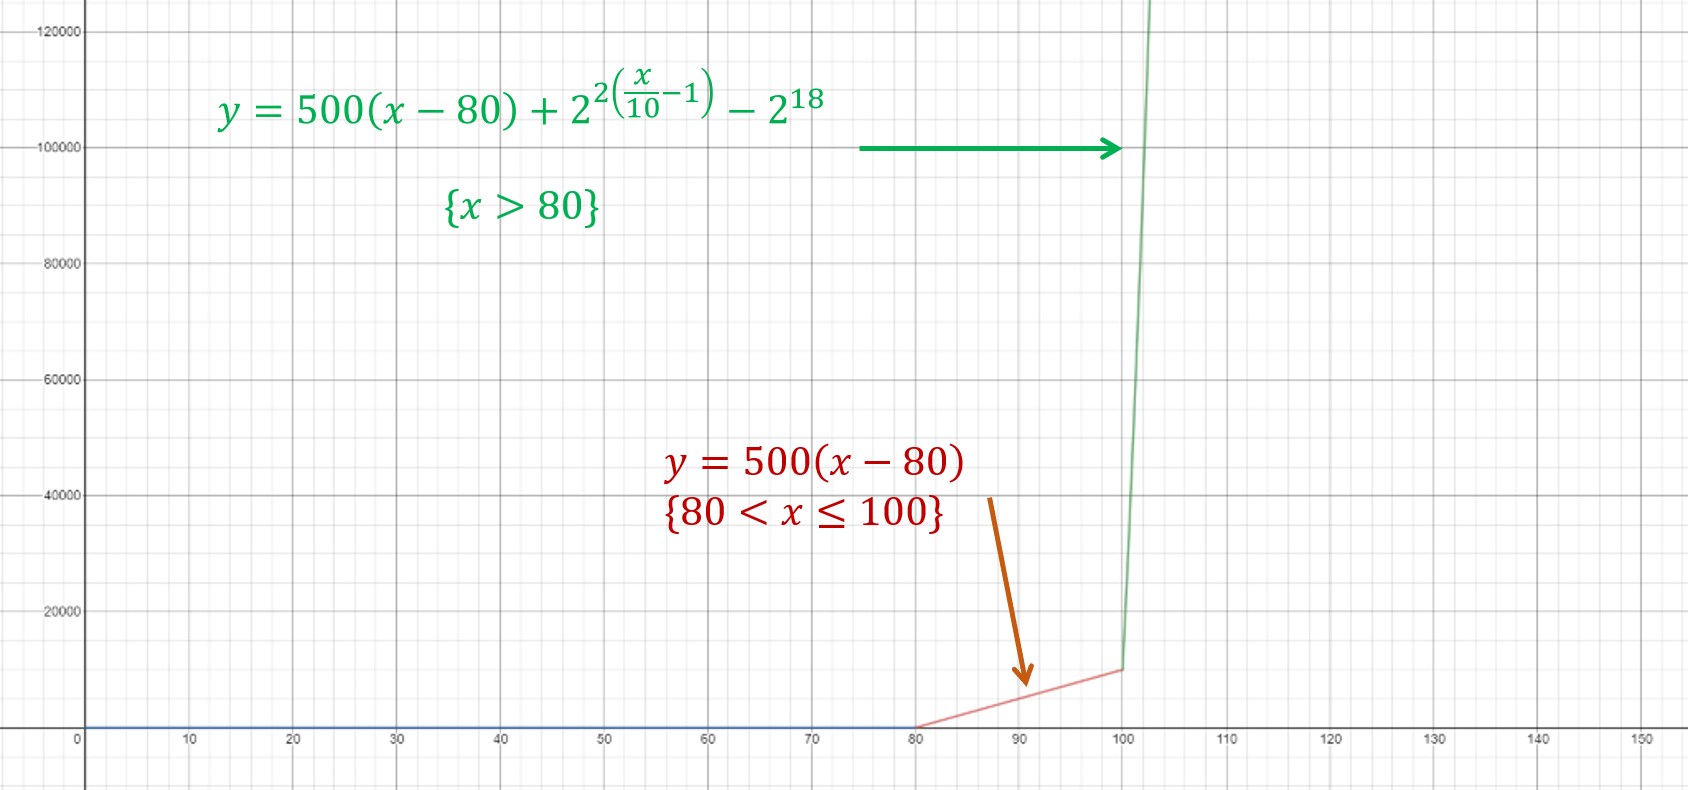
\includegraphics[width=\linewidth]{images/penalty_graph.png}
    \end{center}
    \caption[กราฟแสดงการเพิ่มขึ้นของค่า penalty]{กราฟแสดงการเพิ่มขึ้นของค่า penalty}
    \label{fig:penalty_graph}     
\end{figure}
\CIreply{พูดถึงกรณีนักศึกษาจำนวนมาก เช่น 001102 ว่าจัดการแบบพิเศษกว่าวิชาอื่นอย่างไร}


\section{การประเมินระบบโดยสอบถามความพึงพอใจของนักศึกษา}
\label{sec:ab-eval-design}
ตัวชี้วัดที่ใช้ในการคำนวณ penalty ของตารางสอบที่ได้จากระบบนั้น อาจจะไม่ครอบคลุมความพึงประสงค์ทุกรูปแบบจากนักศึกษา หรือน้ำหนักของตัวชี้วัดที่ใช้ในการคำนวณ penalty นั้นอาจจะเป็นไปได้หลายรูปแบบ
\enskip การสอบถามความพึงพอใจของนักศึกษานั้นจะช่วยในการปรับปรุงอัลกอริทึมเพื่อให้สามารถเลือกใช้น้ำหนักของตัวชี้วัดที่เหมาะสมมากขึ้นในการจัดตารางสอบ
อีกทั้งยังช่วยยืนยันว่าตัวชี้วัดที่โปรแกรมใช้คํานวณค่าความเหมาะสมของตารางสอบนั้นสอดคล้องกับความต้องการของผู้ใช้งาน 
\enskip โดยการประเมินระบบด้วยวิธีการนี้ได้มีการทำ A/B testing\CIreply{cite} โดยได้ออกแบบและสร้างเว็บแอปพลิเคชันให้นักศึกษาผู้ตอบแบบสอบถาม
ล็อกอินผ่าน OAuth ด้วย CMU Account แล้วแสดงข้อมูลตารางสอบของนักศึกษาคนที่ล็อกอิน ภาคการศึกษาละ 2 แบบ เปรียบเทียบกัน 
\CIreply{อ้างอิงรูป screenschot ตรงนี้}
โดยแบบหนึ่งจะเป็นตารางสอบที่กำหนดโดยสำนักทะเบียนและประมวลผล มหาวิทยาลัยเชียงใหม่ 
อีกแบบหนึ่งจะเป็นตารางสอบที่จัดโดยใช้รูปแบบการเรียงลำดับวิชาในการจัดสอบแบบ DEG จากโปรแกรมจัดตารางสอบ
โดยนักศึกษาจะไม่ทราบว่าตารางสอบที่เห็นแต่ละด้านนั้นเป็นแบบใด จากนั้นจะมีแบบฟอร์มให้นักศึกษาเลือกตารางสอบแบบที่ชอบที่สุด แบ่งเป็น 4 ระดับ ได้แก่ (-2) ชอบแบบ A มากที่สุด (-1) ชอบแบบ A มากกว่าเล็กน้อย (0) ชอบทั้งสองแบบเท่า ๆ กัน (1) ชอบแบบ B มากกว่าเล็กน้อย และ (2) ชอบแบบ B มากที่สุด 
โดยหลังจากนำข้อมูลมาประมวลผลแล้ว เราจะกำหนดให้คะแนนที่ติดลบ [-2,-1] บ่งชี้ความพึงพอใจมากกว่าต่อตารางสอบที่กำหนดโดยสำนักทะเบียนและประมวลผล มหาวิทยาลัยเชียงใหม่
คะแนนที่เป็นบวก [1,2] บ่งชี้ความพึงพอใจมากกว่าต่อตารางสอบจากโปรแกรมจัดตารางสอบ โดยนอกจากจะให้นักศึกษาเลือกระดับความพึงพอใจแล้ว นักศึกษายังต้องให้เหตุผลประกอบกับระดับความพึงพอใจที่ตนเองเลือกด้วย

\section{ผลการประเมินระบบด้วย penalty}
การประเมินระบบด้วยค่า penalty นั้นได้มีการจัดตารางสอบทั้งหมด 6 ภาคการศึกษา ตั้งแต่ภาคการศึกษาที่ 1/2561 จนถึงภาคการศึกษาที่ 2/2563
โดยในแต่ละภาคการศึกษาได้มีการทดลองจัดตารางสอบด้วยอัลกอริทึมทั้งหมด 4 รูปแบบ และได้คิดคำนวณจำนวนครั้งที่เกิด penalty และค่า penalty ของตารางสอบแต่ละแบบ ดังตารางที่ \ref{tab:result_table_161}--\ref{tab:result_table_263}
\CIreply{ปี 61 ทำไมไม่มีของสำนักทะเบียน? อธิบายเหตุผลประกอบตรงนี้}
\CIreply{เขียนตีความสรุปผลการประเมิน}
%
\begin{table}[]
    \centering
    \textbf{Total courses: 1432} \quad \quad \textbf{Total students having an exam: 13171}
    \resizebox{\textwidth}{!}{%
    \begin{tabular}{@{}ccrrrrrrrr@{}}
    \toprule
    \textbf{รูปแบบ}                              & \textbf{Penalty}                      & \textbf{1}                & \textbf{2}               & \textbf{3}                   & \textbf{4}                  & \textbf{5}                  & \textbf{6}                  & \textbf{7}                    & \textbf{รวม}                  \\ \midrule
                                                 & \textbf{Count}                        & 0                         & 0                        & 354                          & 430                         & 1854                        & 171                         & 12930                         & 15739                         \\ \cmidrule(l){2-10} 
    \multirow{-2}{*}{BFS-DEG}                    & \textbf{Value}                        & 0                         & 0                        & 27612                        & 33540                       & 70452                       & 4959                        & 155160                        & 291723                        \\ \midrule
                                                 & \textbf{Count}                        & 1                         & 0                        & 480                          & 140                         & 207                         & 71                          & 12038                         & 12937                         \\ \cmidrule(l){2-10} 
    \multirow{-2}{*}{DEG}                        & \textbf{Value}                        & 21                        & 0                        & 37440                        & 10920                       & 7866                        & 2059                        & 144456                        & 202762                        \\ \midrule
                                                 & \textbf{Count}                        & 1                         & 0                        & 588                          & 210                         & 93                          & 69                          & 10465                         & 11426                         \\ \cmidrule(l){2-10} 
    \multirow{-2}{*}{BFS-STD}                    & \textbf{Value}                        & 2                         & 0                        & 45864                        & 16380                       & 3534                        & 2001                        & 125580                        & 193361                        \\ \midrule
    {\color[HTML]{FE0000} }                      & {\color[HTML]{FE0000} \textbf{Count}} & {\color[HTML]{FE0000} 1}  & {\color[HTML]{FE0000} 0} & {\color[HTML]{FE0000} 431}   & {\color[HTML]{FE0000} 116}  & {\color[HTML]{FE0000} 174}  & {\color[HTML]{FE0000} 60}   & {\color[HTML]{FE0000} 8334}   & {\color[HTML]{FE0000} 9116}   \\ \cmidrule(l){2-10} 
    \multirow{-2}{*}{{\color[HTML]{FE0000} STD}} & {\color[HTML]{FE0000} \textbf{Value}} & {\color[HTML]{FE0000} 64} & {\color[HTML]{FE0000} 0} & {\color[HTML]{FE0000} 33618} & {\color[HTML]{FE0000} 9048} & {\color[HTML]{FE0000} 6612} & {\color[HTML]{FE0000} 1740} & {\color[HTML]{FE0000} 100008} & {\color[HTML]{FE0000} 151090} \\ \bottomrule
    \end{tabular}%
    }
    \caption{ตารางแสดงค่า penalty ของตารางสอบภาคการศึกษา 1/2561 ที่จัดสอบ 42 slot}
    \label{tab:result_table_161}
\end{table}
\begin{table}[]
    \centering
    \textbf{Total courses: 1551} \quad \quad \textbf{Total students having an exam: 13095}
    \resizebox{\textwidth}{!}{%
    \begin{tabular}{@{}ccrrrrrrrr@{}}
    \toprule
    \textbf{รูปแบบ}                              & \textbf{Penalty}                      & \textbf{1}                  & \textbf{2}               & \textbf{3}                   & \textbf{4}                   & \textbf{5}                   & \textbf{6}                  & \textbf{7}                    & \textbf{รวม}                  \\ \midrule
                                                 & \textbf{Count}                        & 1                           & 0                        & 1050                         & 583                          & 296                          & 314                         & 10977                         & 13221                         \\ \cmidrule(l){2-10} 
    \multirow{-2}{*}{BFS-DEG}                    & \textbf{Value}                        & 2467                        & 0                        & 81900                        & 45474                        & 11248                        & 9106                        & 131724                        & 281919                        \\ \midrule
                                                 & \textbf{Count}                        & 1                           & 0                        & 884                          & 264                          & 398                          & 242                         & 12158                         & 13947                         \\ \cmidrule(l){2-10} 
    \multirow{-2}{*}{DEG}                        & \textbf{Value}                        & 238                         & 0                        & 68952                        & 20592                        & 15124                        & 7018                        & 145896                        & 257820                        \\ \midrule
                                                 & \textbf{Count}                        & 1                           & 0                        & 1343                         & 374                          & 742                          & 208                         & 10342                         & 13010                         \\ \cmidrule(l){2-10} 
    \multirow{-2}{*}{BFS-STD}                    & \textbf{Value}                        & 2                           & 0                        & 104754                       & 29172                        & 28196                        & 6032                        & 124104                        & 292260                        \\ \midrule
    {\color[HTML]{FE0000} }                      & {\color[HTML]{FE0000} \textbf{Count}} & {\color[HTML]{FE0000} 1}    & {\color[HTML]{FE0000} 0} & {\color[HTML]{FE0000} 814}   & {\color[HTML]{FE0000} 247}   & {\color[HTML]{FE0000} 266}   & {\color[HTML]{FE0000} 203}  & {\color[HTML]{FE0000} 9649}   & {\color[HTML]{FE0000} 11180}  \\ \cmidrule(l){2-10} 
    \multirow{-2}{*}{{\color[HTML]{FE0000} STD}} & {\color[HTML]{FE0000} \textbf{Value}} & {\color[HTML]{FE0000} 2251} & {\color[HTML]{FE0000} 0} & {\color[HTML]{FE0000} 63492} & {\color[HTML]{FE0000} 19266} & {\color[HTML]{FE0000} 10108} & {\color[HTML]{FE0000} 5887} & {\color[HTML]{FE0000} 115788} & {\color[HTML]{FE0000} 216792} \\ \bottomrule
    \end{tabular}%
    }
    \caption{ตารางแสดงค่า penalty ของตารางสอบภาคการศึกษา 2/2561 ที่จัดสอบ 42 slot}
    \label{tab:result_table_261}
\end{table}
\begin{table}[]
    \centering
    \textbf{Total courses: 1729} \quad \quad \textbf{Total students having an exam: 19786}
    \resizebox{\textwidth}{!}{%
    \begin{tabular}{@{}ccrrrrrrrr@{}}
    \toprule
    \textbf{รูปแบบ}                              & \textbf{Penalty}                      & \textbf{1}                  & \textbf{2}               & \textbf{3}                   & \textbf{4}                   & \textbf{5}                   & \textbf{6}                  & \textbf{7}                    & \textbf{รวม}                  \\ \midrule
                                                 & \textbf{Count}                        & 0                           & 0                        & 1110                         & 657                          & 1217                         & 639                         & 18036                         & 21659                         \\ \cmidrule(l){2-10} 
    \multirow{-2}{*}{BFS-DEG}                    & \textbf{Value}                        & 0                           & 0                        & 86580                        & 51246                        & 46246                        & 18531                       & 216432                        & 419035                        \\ \midrule
                                                 & \textbf{Count}                        & 1                           & 0                        & 1155                         & 242                          & 522                          & 147                         & 18859                         & 20926                         \\ \cmidrule(l){2-10} 
    \multirow{-2}{*}{DEG}                        & \textbf{Value}                        & 714                         & 0                        & 90090                        & 18876                        & 19836                        & 4263                        & 226308                        & 360087                        \\ \midrule
                                                 & \textbf{Count}                        & 1                           & 0                        & 1500                         & 595                          & 259                          & 159                         & 15990                         & 18504                         \\ \cmidrule(l){2-10} 
    \multirow{-2}{*}{BFS-STD}                    & \textbf{Value}                        & 2                           & 0                        & 117000                       & 46410                        & 9842                         & 4611                        & 191880                        & 369745                        \\ \midrule
    {\color[HTML]{FE0000} }                      & {\color[HTML]{FE0000} \textbf{Count}} & {\color[HTML]{FE0000} 3}    & {\color[HTML]{FE0000} 0} & {\color[HTML]{FE0000} 965}   & {\color[HTML]{FE0000} 334}   & {\color[HTML]{FE0000} 337}   & {\color[HTML]{FE0000} 231}  & {\color[HTML]{FE0000} 15535}  & {\color[HTML]{FE0000} 17405}  \\ \cmidrule(l){2-10} 
    \multirow{-2}{*}{{\color[HTML]{FE0000} STD}} & {\color[HTML]{FE0000} \textbf{Value}} & {\color[HTML]{FE0000} 4259} & {\color[HTML]{FE0000} 0} & {\color[HTML]{FE0000} 75270} & {\color[HTML]{FE0000} 26052} & {\color[HTML]{FE0000} 12806} & {\color[HTML]{FE0000} 6699} & {\color[HTML]{FE0000} 186420} & {\color[HTML]{FE0000} 311506} \\ \midrule
                                                 & \textbf{Count}                        & 0                           & 3247                     & 3406                         & 2333                         & 7663                         & 5863                        & 18667                         & 41179                         \\ \cmidrule(l){2-10} 
    \multirow{-2}{*}{สำนักทะเบียน}                  & \textbf{Value}                        & 0                           & 32470000                 & 265668                       & 181974                       & 291194                       & 170027                      & 224004                        & 33602867                      \\ \bottomrule
    \end{tabular}%
    }
    \caption{ตารางแสดงค่า penalty ของตารางสอบภาคการศึกษา 1/2562 ที่จัดสอบ 42 slot}
    \label{tab:result_table_162}
\end{table}
\begin{table}[]
    \centering
    \textbf{Total courses: 1828} \quad \quad \textbf{Total students having an exam: 19505}
    \resizebox{\textwidth}{!}{%
    \begin{tabular}{@{}ccrrrrrrrr@{}}
    \toprule
    \textbf{รูปแบบ}                              & \textbf{Penalty}                      & \textbf{1}                 & \textbf{2}               & \textbf{3}                    & \textbf{4}                   & \textbf{5}                   & \textbf{6}                  & \textbf{7}                    & \textbf{รวม}                  \\ \midrule
                                                 & \textbf{Count}                        & 1                          & 0                        & 1624                          & 1072                         & 1460                         & 883                         & 16578                         & 21618                         \\ \cmidrule(l){2-10} 
    \multirow{-2}{*}{BFS-DEG}                    & \textbf{Value}                        & 11907                      & 0                        & 126672                        & 83616                        & 55480                        & 25607                       & 198936                        & 502218                        \\ \midrule
                                                 & \textbf{Count}                        & 1                          & 0                        & 1045                          & 374                          & 262                          & 138                         & 19168                         & 20988                         \\ \cmidrule(l){2-10} 
    \multirow{-2}{*}{DEG}                        & \textbf{Value}                        & 545                        & 0                        & 81510                         & 29172                        & 9956                         & 4002                        & 230016                        & 355201                        \\ \midrule
                                                 & \textbf{Count}                        & 0                          & 0                        & 1732                          & 864                          & 785                          & 448                         & 16085                         & 19914                         \\ \cmidrule(l){2-10} 
    \multirow{-2}{*}{BFS-STD}                    & \textbf{Value}                        & 0                          & 0                        & 135096                        & 67392                        & 29830                        & 12992                       & 193020                        & 438330                        \\ \midrule
    {\color[HTML]{FE0000} }                      & {\color[HTML]{FE0000} \textbf{Count}} & {\color[HTML]{FE0000} 1}   & {\color[HTML]{FE0000} 0} & {\color[HTML]{FE0000} 1303}   & {\color[HTML]{FE0000} 250}   & {\color[HTML]{FE0000} 343}   & {\color[HTML]{FE0000} 192}  & {\color[HTML]{FE0000} 14545}  & {\color[HTML]{FE0000} 16634}  \\ \cmidrule(l){2-10} 
    \multirow{-2}{*}{{\color[HTML]{FE0000} STD}} & {\color[HTML]{FE0000} \textbf{Value}} & {\color[HTML]{FE0000} 497} & {\color[HTML]{FE0000} 0} & {\color[HTML]{FE0000} 101634} & {\color[HTML]{FE0000} 19500} & {\color[HTML]{FE0000} 13034} & {\color[HTML]{FE0000} 5568} & {\color[HTML]{FE0000} 174540} & {\color[HTML]{FE0000} 314773} \\ \midrule
                                                 & \textbf{Count}                        & 1                          & 4732                     & 3908                          & 2608                         & 5757                         & 5157                        & 18698                         & 40861                         \\ \cmidrule(l){2-10} 
    \multirow{-2}{*}{สำนักทะเบียน}                  & \textbf{Value}                        & 24129                      & 47320000                 & 304824                        & 203424                       & 218766                       & 149553                      & 224376                        & 48445072                      \\ \bottomrule
    \end{tabular}%
    }
    \caption{ตารางแสดงค่า penalty ของตารางสอบภาคการศึกษา 2/2562 ที่จัดสอบ 42 slot}
    \label{tab:result_table_262}
\end{table}
\begin{table}[]
    \centering
    \textbf{Total courses: 1894} \quad \quad \textbf{Total students having an exam: 26549}
    \resizebox{\textwidth}{!}{%
    \begin{tabular}{@{}ccrrrrrrrr@{}}
    \toprule
    \textbf{รูปแบบ}                              & \textbf{Penalty}                      & \textbf{1}                  & \textbf{2}               & \textbf{3}                    & \textbf{4}                   & \textbf{5}                   & \textbf{6}                  & \textbf{7}                    & \textbf{รวม}                  \\ \midrule
                                                 & \textbf{Count}                        & 2                           & 0                        & 1717                          & 681                          & 511                          & 524                         & 21515                         & 24950                         \\ \cmidrule(l){2-10} 
    \multirow{-2}{*}{BFS-DEG}                    & \textbf{Value}                        & 5633                        & 0                        & 133926                        & 53118                        & 19418                        & 15196                       & 258180                        & 485471                        \\ \midrule
                                                 & \textbf{Count}                        & 2                           & 0                        & 1722                          & 673                          & 506                          & 511                         & 22860                         & 26274                         \\ \cmidrule(l){2-10} 
    \multirow{-2}{*}{DEG}                        & \textbf{Value}                        & 6568                        & 0                        & 134316                        & 52494                        & 19228                        & 14819                       & 274320                        & 501745                        \\ \midrule
                                                 & \textbf{Count}                        & 2                           & 0                        & 1722                          & 654                          & 486                          & 293                         & 23154                         & 26311                         \\ \cmidrule(l){2-10} 
    \multirow{-2}{*}{BFS-STD}                    & \textbf{Value}                        & 3856                        & 0                        & 134316                        & 51012                        & 18468                        & 8497                        & 277848                        & 493997                        \\ \midrule
    {\color[HTML]{FE0000} }                      & {\color[HTML]{FE0000} \textbf{Count}} & {\color[HTML]{FE0000} 2}    & {\color[HTML]{FE0000} 0} & {\color[HTML]{FE0000} 1556}   & {\color[HTML]{FE0000} 681}   & {\color[HTML]{FE0000} 563}   & {\color[HTML]{FE0000} 286}  & {\color[HTML]{FE0000} 20888}  & {\color[HTML]{FE0000} 23976}  \\ \cmidrule(l){2-10} 
    \multirow{-2}{*}{{\color[HTML]{FE0000} STD}} & {\color[HTML]{FE0000} \textbf{Value}} & {\color[HTML]{FE0000} 1252} & {\color[HTML]{FE0000} 0} & {\color[HTML]{FE0000} 121368} & {\color[HTML]{FE0000} 53118} & {\color[HTML]{FE0000} 21394} & {\color[HTML]{FE0000} 8294} & {\color[HTML]{FE0000} 250656} & {\color[HTML]{FE0000} 456082} \\ \midrule
                                                 & \textbf{Count}                        & 0                           & 4983                     & 3786                           & 3498                           & 8676                           & 7784                   & 26703                         & 55430                         \\ \cmidrule(l){2-10} 
    \multirow{-2}{*}{สำนักทะเบียน}                  & \textbf{Value}                        & 0                           & 49830000                 & 295308                         & 272844                         & 329688                         & 225736                 & 320436                        & 51274012                      \\ \bottomrule
    \end{tabular}%
    }
    \caption{ตารางแสดงค่า penalty ของตารางสอบภาคการศึกษา 1/2563 ที่จัดสอบ 42 slot}
    \label{tab:result_table_163}
\end{table}
\begin{table}[]
    \centering
    \textbf{Total courses: 1770} \quad \quad \textbf{Total students having an exam: 24392}
    \resizebox{\textwidth}{!}{%
    \begin{tabular}{@{}ccrrrrrrrr@{}}
    \toprule
    \textbf{รูปแบบ}                              & \textbf{Penalty}                      & \textbf{1}               & \textbf{2}               & \textbf{3}                    & \textbf{4}                   & \textbf{5}                   & \textbf{6}                   & \textbf{7}                    & \textbf{รวม}                  \\ \midrule
                                                 & \textbf{Count}                        & 1                        & 0                        & 2537                          & 747                          & 666                          & 616                          & 22015                         & 26582                         \\ \cmidrule(l){2-10} 
    \multirow{-2}{*}{BFS-DEG}                    & \textbf{Value}                        & 4                        & 0                        & 197886                        & 58266                        & 25308                        & 17864                        & 264180                        & 563508                        \\ \midrule
    {\color[HTML]{FE0000} }                      & {\color[HTML]{FE0000} \textbf{Count}} & {\color[HTML]{FE0000} 1} & {\color[HTML]{FE0000} 0} & {\color[HTML]{FE0000} 1709}   & {\color[HTML]{FE0000} 711}   & {\color[HTML]{FE0000} 693}   & {\color[HTML]{FE0000} 575}   & {\color[HTML]{FE0000} 21042}  & {\color[HTML]{FE0000} 24731}  \\ \cmidrule(l){2-10} 
    \multirow{-2}{*}{{\color[HTML]{FE0000} DEG}} & {\color[HTML]{FE0000} \textbf{Value}} & {\color[HTML]{FE0000} 1} & {\color[HTML]{FE0000} 0} & {\color[HTML]{FE0000} 133302} & {\color[HTML]{FE0000} 55458} & {\color[HTML]{FE0000} 26334} & {\color[HTML]{FE0000} 16675} & {\color[HTML]{FE0000} 252504} & {\color[HTML]{FE0000} 484274} \\ \midrule
                                                 & \textbf{Count}                        & 1                        & 0                        & 2011                          & 1612                         & 743                          & 474                          & 24440                         & 29281                         \\ \cmidrule(l){2-10} 
    \multirow{-2}{*}{BFS-STD}                    & \textbf{Value}                        & 4                        & 0                        & 156858                        & 125736                       & 28234                        & 13746                        & 293280                        & 617858                        \\ \midrule
                                                 & \textbf{Count}                        & 0                        & 1                        & 1862                          & 717                          & 515                          & 342                          & 21313                         & 24750                         \\ \cmidrule(l){2-10} 
    \multirow{-2}{*}{STD}                        & \textbf{Value}                        & 0                        & 10000                    & 145236                        & 55926                        & 19570                        & 9918                         & 255756                        & 496406                        \\ \midrule
                                                 & \textbf{Count}                        & 2                        & 4128                     & 3224                          & 6477                         & 7468                         & 4206                         & 25640                         & 51145                         \\ \cmidrule(l){2-10} 
    \multirow{-2}{*}{สำนักทะเบียน}               & \textbf{Value}                          & 333067582                 & 41280000                 & 251472                        & 505206                       & 283784                       & 121974                       & 307680                        & 375817698                     \\ \bottomrule
    \end{tabular}%
    }
    \caption{ตารางแสดงค่า penalty ของตารางสอบภาคการศึกษา 2/2563 ที่จัดสอบ 42 slot}
    \label{tab:result_table_263}
\end{table}

\section{ผลการประเมินระบบโดยสอบถามความพึงพอใจของนักศึกษา}
\subsection{การออกแบบส่วนแสดงผลผู้ใช้งาน}
\CIreply{ย้ายไป~\ref{sec:ab-eval-design}}
ส่วนแสดงผลสำหรับผู้ใช้งานจะมีหน้าหลัก ๆ อยู่ทั้งหมด 2 หน้า โดยมีหน้าแรกสำหรับแจ้งคำอธิบายการใช้งานและล็อกอิน ดังรูปที่ \ref{fig:eval_ui_1}
และหน้าสำหรับแสดงตารางสอบพร้อมด้วยแบบฟอร์มสำหรับเลือกระดับความพึงพอใจและกรอกความคิดเห็นเพิ่มเติม ดังรูปที่ \ref{fig:eval_ui_2}
\CIreply{ใส่ screenshot Google Forms?}
\begin{figure}
    \begin{center}
      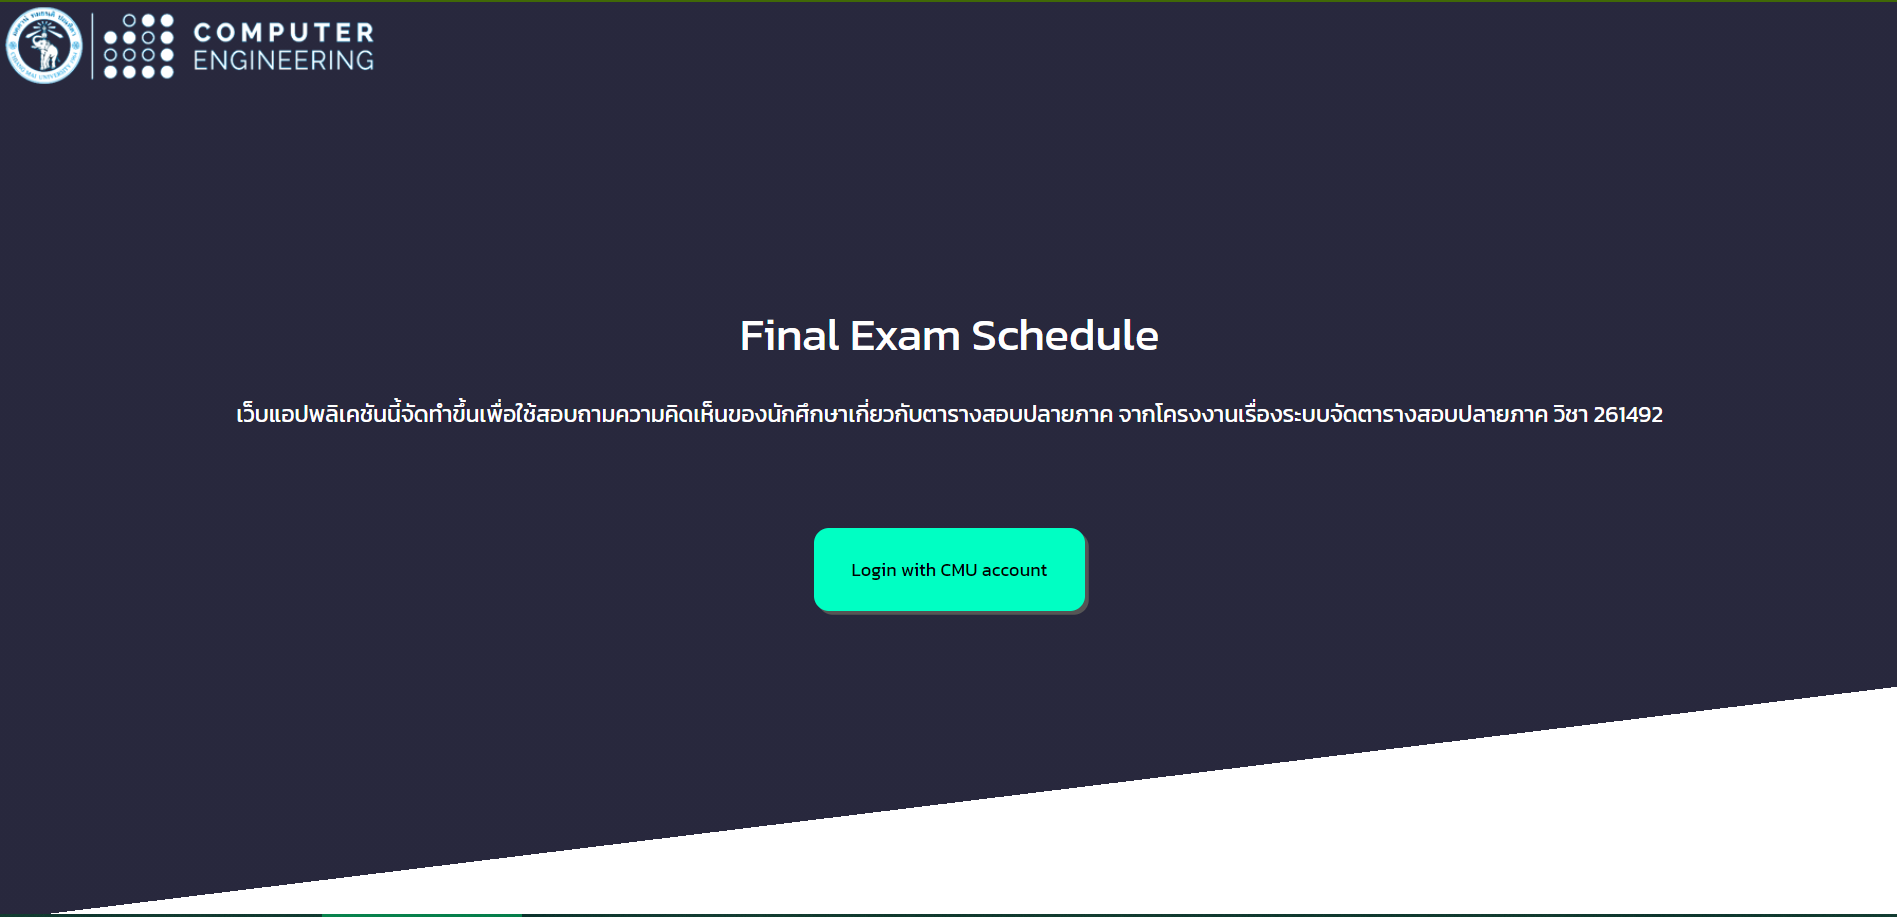
\includegraphics[width=\linewidth]{images/eval_ui_1.png}
    \end{center}
    \caption[UI หน้า Home ของเว็บแอปพลิเคชัน]{UI หน้า Home ของเว็บแอปพลิเคชัน}
    \label{fig:eval_ui_1}     
\end{figure}
\begin{figure}
    \begin{center}
      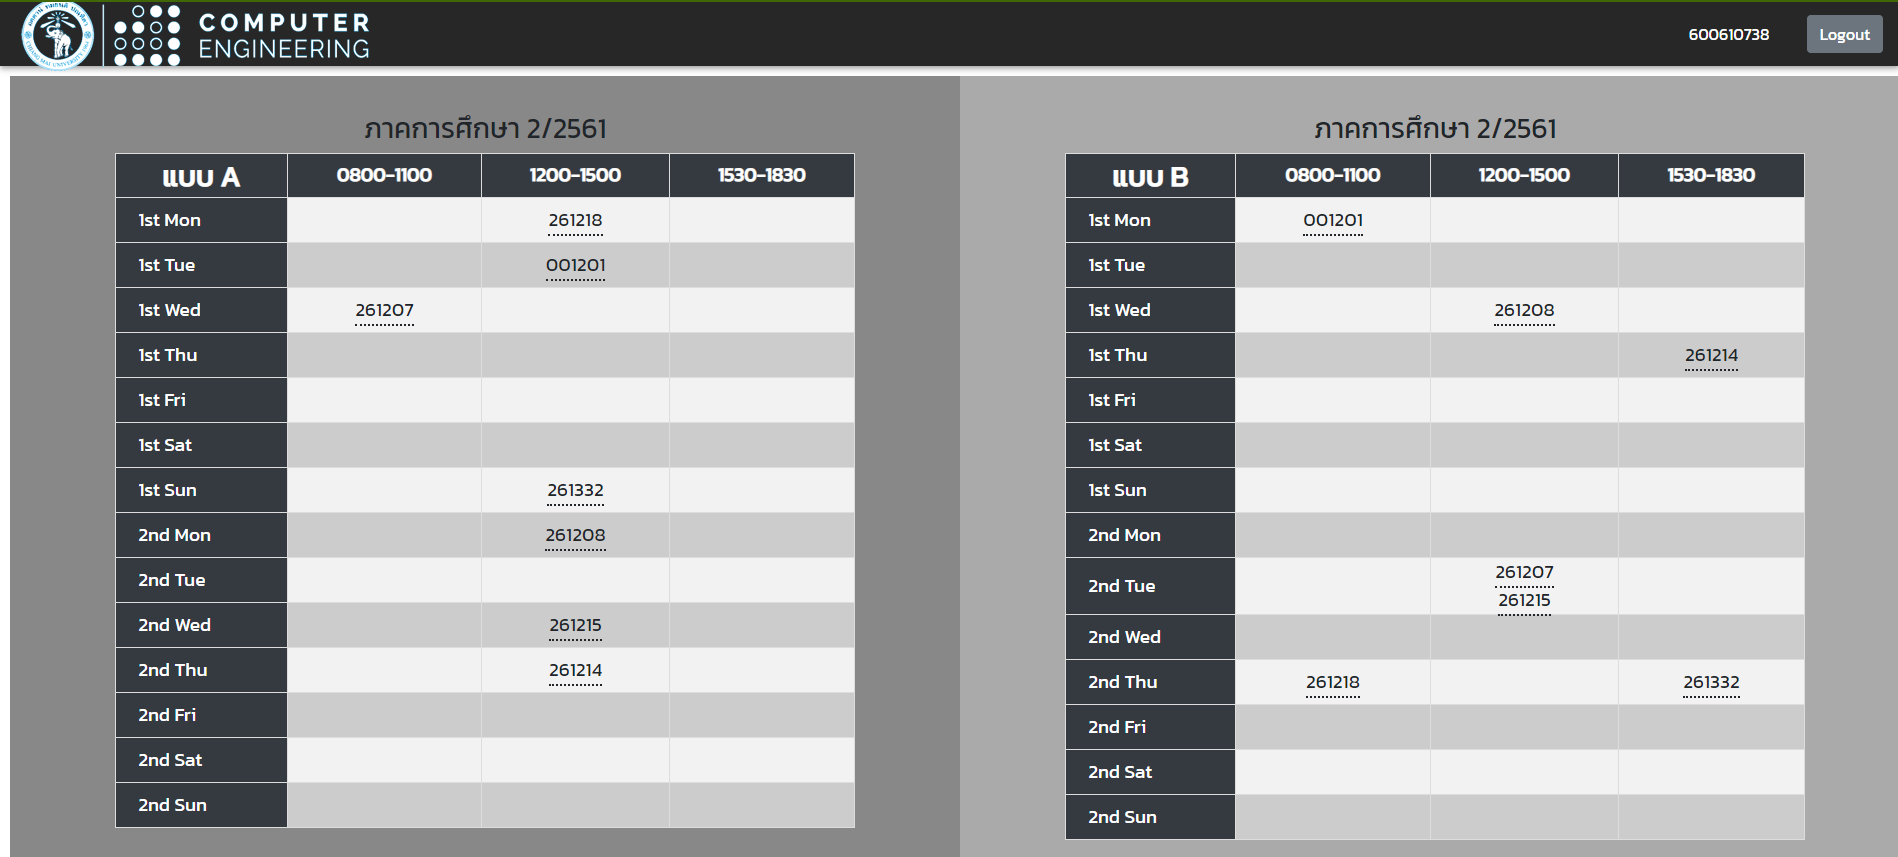
\includegraphics[width=\linewidth]{images/eval_ui_2.png}
    \end{center}
    \caption[UI หน้าแสดงตารางสอบสำหรับใช้ในการเปรียบเทียบ]{UI หน้าแสดงตารางสอบสำหรับใช้ในการเปรียบเทียบ}
    \label{fig:eval_ui_2}     
\end{figure}

\subsection{ผลจากแบบสอบถามความพึงพอใจของนักศึกษา}
ผลการประเมินระบบโดยสอบถามความพึงพอใจของนักศึกษา ด้วยวิธีการทำ A/B testing 
โดยให้นักศึกษาเปรียบเทียบและเลือกตารางสอบที่ตนเองชอบจากตารางสอบสองแบบ โดยแบบหนึ่งเป็นตารางสอบจากสำนักทะเบียนและประมวลผล มหาวิทยาลัยเชียงใหม่ 
อีกแบบเป็นตารางสอบที่ดีที่สุดจากทุกรูปแบบที่จัดโดยโปรแกรม โดยนักศึกษาที่ทำแบบสำรวจจะไม่ทราบว่าตารางสอบที่ตนเองเห็นเป็นตารางสอบแบบใดนั้น 
ได้รับผลการตอบกลับแบบฟอร์มทั้งหมด 688 ครั้ง จากนักศึกษาจำนวน 180 คน
โดยพบว่า จากผลการสำรวจ นักศึกษามากกว่า 61\% ชอบตารางสอบที่จัดโดยโปรแกรมมากกว่าตารางสอบที่กำหนดโดยสำนักทะเบียนและประมวลผล มหาวิทยาลัยเชียงใหม่
โดยผลการนับจำนวนนักศึกษาที่เลือกระดับความพึงพอใจในตารางสอบแต่ละแบบ มีค่าเฉลี่ยความพึงพอใจเท่ากับ 0.59 และมีค่า standard deviation เท่ากับ 1.57 
โดยสามารถแจกแจงจำนวนครั้งสำหรับแต่ละระดับความพึงพอใจได้ดังรูปที่ \ref{fig:eval_result_1} และหากแจกแจงแยกตามภาคการศึกษาจะแสดงได้ดังตารางที่ \ref{tab:eval_result_2} 
\CIreply{เขียนสรุปแจกแจงจำนวนนักศึกษาจากแต่ละคณะ}
\CIreply{เขียนสรุปตีความผลการสำรวจ}
\CIreply{ในตาราง หากมีหลาย slots อย่าลืมเติม s}
\begin{figure}
    \begin{center}
      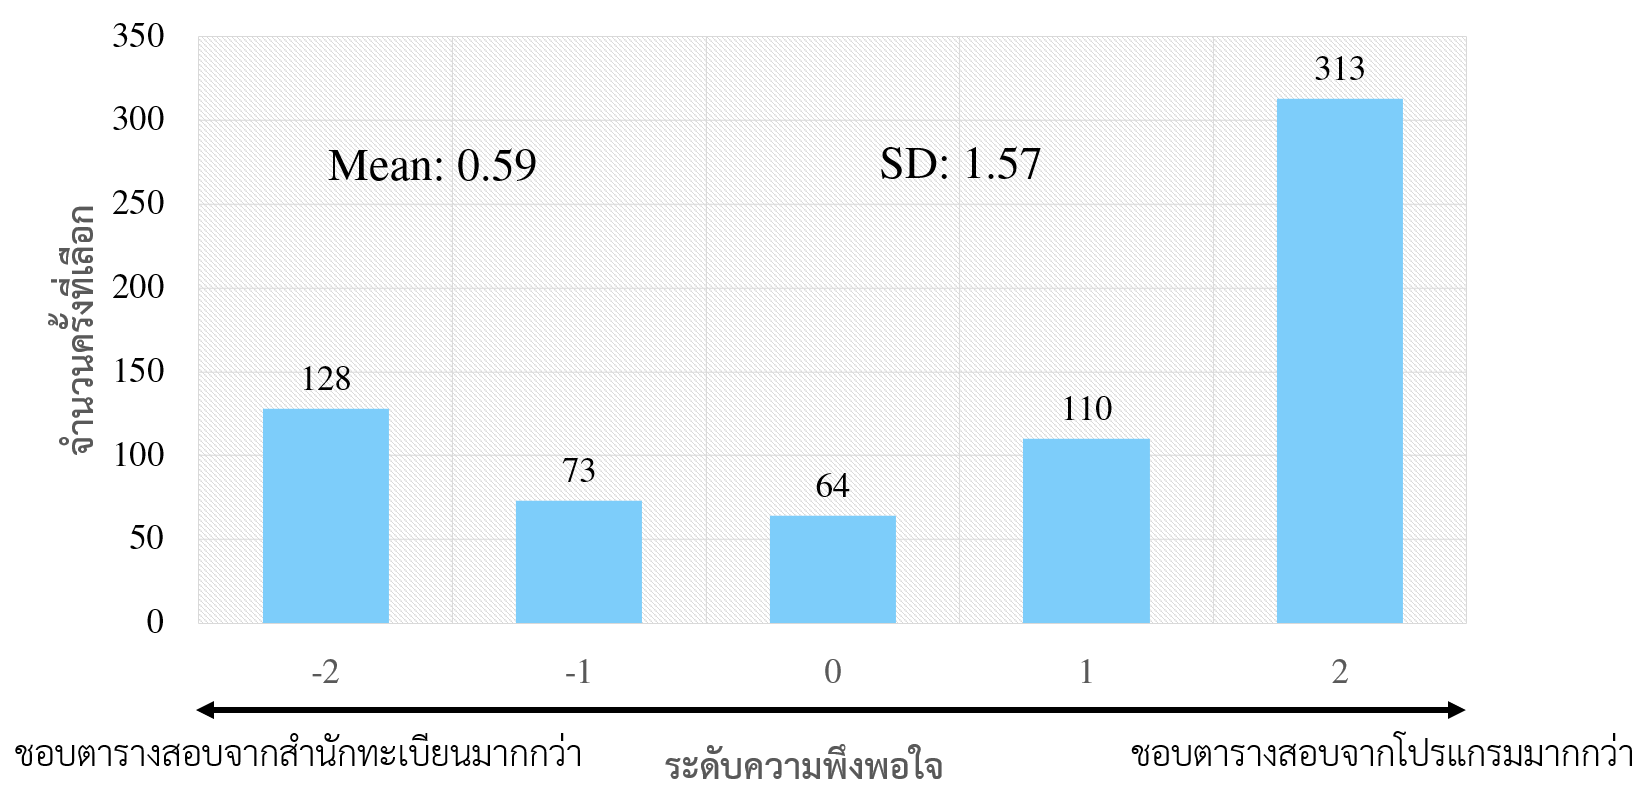
\includegraphics[width=\linewidth]{images/eval_result_1.png}
    \end{center}
    \caption[กราฟแสดงจำนวนครั้งในแต่ละระดับความพึงพอใจของนักศึกษาต่อตารางสอบ]{กราฟแสดงจำนวนครั้งในแต่ละระดับความพึงพอใจของนักศึกษาต่อตารางสอบ}
    \label{fig:eval_result_1}     
\end{figure}
\begin{table}[]
    \centering
    % \resizebox{.6\textwidth}{!}{%
    \begin{tabular}{@{}cccccc@{}}
    \toprule
                               & \multicolumn{5}{c}{Total Counts of}                                                                                                         \\ \cmidrule(l){2-6} 
    \multirow{-2}{*}{Semester} & \cellcolor[HTML]{F8696B}-2 & \cellcolor[HTML]{FAB2B5}-1 & \cellcolor[HTML]{FCFCFF}0 & \cellcolor[HTML]{B0DDBD}1 & \cellcolor[HTML]{63BE7B}2 \\ \midrule
    1/2561                     & 16                         & 15                         & 16                        & 23                        & 40                        \\
    2/2561                     & 20                         & 9                          & 5                         & 14                        & 34                        \\
    1/2562                     & 20                         & 12                         & 11                        & 10                        & 59                        \\
    2/2562                     & 15                         & 8                          & 5                         & 20                        & 65                        \\
    1/2563                     & 28                         & 15                         & 10                        & 28                        & 59                        \\
    2/2563                     & 29                         & 14                         & 17                        & 15                        & 56                        \\ \bottomrule
    \end{tabular}%
    % }
    \caption{แสดงการแจกแจงจำนวนครั้งสำหรับแต่ละระดับความพึงพอใจแบ่งตามภาคการศึกษา}
    \label{tab:eval_result_2}
\end{table}

\section{การทดลองลดช่วงเวลาในการจัดสอบ}
นอกจากการทดลองจัดตารางสอบในแต่ละภาคการศึกษาที่ผ่านมา ด้วยจำนวนช่วงเวลาสอบ 42 slots หรือ 14 วัน วันละ 3 slots แล้ว
เรายังได้ทำการทดลองลดช่วงเวลาในการจัดสอบลงจาก 42 slots ให้เหลือ 36 33 และ 28 slots ตามลำดับ
เพื่อดูแนวโน้มในการเพิ่มขึ้นของจำนวนครั้งที่มีนักศึกษาสอบสองวิชาในเวลาเดียวกันจาก\CI{รูปแบบการจัดเรียง}{เรามีชื่อเรียก variations พวกนี้โดยรวมหรือไม่ ถ้ามีก็ควรใช้ให้เสมอต้นเสมอปลาย ถ้าไม่มีก็ตั้งขึ้นมาให้ชัดเจน}แบบต่าง ๆ เปรียบเทียบกัน
โดยได้ผลจำนวนครั้งที่มีนักศึกษาสอบสองวิชาในเวลาเดียวกันในแต่ละภาคการศึกษาและแต่ละรูปแบบการจัดเรียง ดังตารางที่ \ref{tab:overlap_count_result}
และได้ผลลัพธ์จากการคำนวณค่า penalty ของตารางสอบแต่ละภาคการศึกษา ที่จัดโดยกำหนดจำนวนช่วงเวลาในการจัดสอบต่าง ๆ กัน ดังนี้
\begin{itemize}
    \item กำหนดช่วงเวลาในการจัดสอบ 36 slot แสดงดังตารางที่ \ref{tab:result_table_161_36}--\ref{tab:result_table_263_36}
    \item กำหนดช่วงเวลาในการจัดสอบ 33 slot แสดงดังตารางที่ \ref{tab:result_table_161_33}--\ref{tab:result_table_263_33}
    \item กำหนดช่วงเวลาในการจัดสอบ 28 slot แสดงดังตารางที่ \ref{tab:result_table_161_28}--\ref{tab:result_table_263_28}
\end{itemize}
ซึ่งจากผลลัพธ์จากตารางที่ \ref{tab:overlap_count_result} จะสามารถสรุปได้ว่ารูปแบบการเรียงลำดับความสำคัญในการจัดช่วงเวลาสอบให้กับวิชารูปแบบ DEG นั้น 
มีแนวโน้มที่จะจัดตารางสอบแล้วทำให้โอกาสการเกิดสถานการณ์ที่นักศึกษามีสอบสองวิชาในเวลาเดียวกันเกิดขึ้นได้น้อยที่สุด
\CIreply{สรุปด้วยว่าเราสามารถลดจำนวน slots ได้มากน้อยเพียงใด}
\begin{table}[]
    \centering
    \begin{tabular}{@{}ccrrrr@{}}
    \toprule
                                  &                            & \multicolumn{4}{c}{จำนวน slot สอบ}                                                                         \\ \cmidrule(l){3-6} 
    \multirow{-2}{*}{ภาคการศึกษา} & \multirow{-2}{*}{รูปแบบ}   & 28                        & 33                       & 36                       & 42                       \\ \midrule
                                  & BFS-DEG                    & 3                         & 7                        & 3                        & 0                        \\ \cmidrule(l){2-6} 
                                  & {\color[HTML]{FE0000} DEG} & {\color[HTML]{FE0000} 0}  & {\color[HTML]{FE0000} 0} & {\color[HTML]{FE0000} 0} & {\color[HTML]{FE0000} 0} \\ \cmidrule(l){2-6} 
                                  & BFS-STD                    & 0                         & 0                        & 0                        & 0                        \\ \cmidrule(l){2-6} 
    \multirow{-4}{*}{1/2561}      & STD                        & 2                         & 0                        & 0                        & 0                        \\ \midrule
                                  & BFS-DEG                    & 24                        & 0                        & 1                        & 0                        \\ \cmidrule(l){2-6} 
                                  & {\color[HTML]{FE0000} DEG} & {\color[HTML]{FE0000} 2}  & {\color[HTML]{FE0000} 0} & {\color[HTML]{FE0000} 0} & {\color[HTML]{FE0000} 0} \\ \cmidrule(l){2-6} 
                                  & BFS-STD                    & 34                        & 8                        & 1                        & 0                        \\ \cmidrule(l){2-6} 
    \multirow{-4}{*}{2/2561}      & STD                        & 15                        & 4                        & 1                        & 0                        \\ \midrule
                                  & BFS-DEG                    & 74                        & 0                        & 5                        & 0                        \\ \cmidrule(l){2-6} 
                                  & {\color[HTML]{FE0000} DEG} & {\color[HTML]{FE0000} 2}  & {\color[HTML]{FE0000} 0} & {\color[HTML]{FE0000} 0} & {\color[HTML]{FE0000} 0} \\ \cmidrule(l){2-6} 
                                  & BFS-STD                    & 14                        & 0                        & 0                        & 0                        \\ \cmidrule(l){2-6} 
    \multirow{-4}{*}{1/2562}      & STD                        & 26                        & 5                        & 0                        & 0                        \\ \midrule
                                  & BFS-DEG                    & 286                       & 149                      & 42                       & 0                        \\ \cmidrule(l){2-6} 
                                  & {\color[HTML]{FE0000} DEG} & {\color[HTML]{FE0000} 6}  & {\color[HTML]{FE0000} 0} & {\color[HTML]{FE0000} 0} & {\color[HTML]{FE0000} 0} \\ \cmidrule(l){2-6} 
                                  & BFS-STD                    & 34                        & 1                        & 4                        & 0                        \\ \cmidrule(l){2-6} 
    \multirow{-4}{*}{2/2562}      & STD                        & 54                        & 7                        & 5                        & 0                        \\ \midrule
                                  & BFS-DEG                    & 25                        & 1                        & 0                        & 0                        \\ \cmidrule(l){2-6} 
                                  & {\color[HTML]{FE0000} DEG} & {\color[HTML]{FE0000} 25} & {\color[HTML]{FE0000} 1} & {\color[HTML]{FE0000} 0} & {\color[HTML]{FE0000} 0} \\ \cmidrule(l){2-6} 
                                  & BFS-STD                    & 65                        & 12                       & 2                        & 0                        \\ \cmidrule(l){2-6} 
    \multirow{-4}{*}{1/2563}      & STD                        & 50                        & 16                       & 8                        & 0                        \\ \midrule
                                  & BFS-DEG                    & 56                        & 19                       & 0                        & 0                        \\ \cmidrule(l){2-6} 
                                  & {\color[HTML]{FE0000} DEG} & {\color[HTML]{FE0000} 17} & {\color[HTML]{FE0000} 1} & {\color[HTML]{FE0000} 0} & {\color[HTML]{FE0000} 0} \\ \cmidrule(l){2-6} 
                                  & BFS-STD                    & 66                        & 9                        & 2                        & 0                        \\ \cmidrule(l){2-6} 
    \multirow{-4}{*}{2/2563}      & STD                        & 47                        & 10                       & 2                        & 1                        \\ \bottomrule
    \end{tabular}
    \caption{ตารางแสดงจำนวนครั้งที่มีนักศึกษาสอบสองวิชาในเวลาเดียวกัน}
    \label{tab:overlap_count_result}
    \end{table}
\begin{table}[]
    \centering
    \textbf{Total courses: 1432} \quad \quad \textbf{Total students having an exam: 13171}
    \resizebox{\textwidth}{!}{%
    \begin{tabular}{@{}ccrrrrrrrr@{}}
    \toprule
    \textbf{รูปแบบ}                              & \textbf{Penalty}                      & \textbf{1}                  & \textbf{2}                    & \textbf{3}                    & \textbf{4}                    & \textbf{5}                    & \textbf{6}                   & \textbf{7}                    & \textbf{รวม}                  \\ \midrule
                                                & \textbf{Count}                        & 0                              & 3                              & 822                            & 1009                           & 1090                           & 553                            & 6578                           & 10055                            \\ \cmidrule(l){2-10} 
    \multirow{-2}{*}{BFS-DEG}                   & \textbf{Value}                        & 0                              & 30000                          & 64116                          & 78702                          & 41420                          & 16037                          & 78936                          & 309211                           \\ \midrule
                                                & \textbf{Count}                        & 0                              &  0                             &  997                           &  202                           & 548                            &  136                           &  8029                          & 9912      \\ \cmidrule(l){2-10} 
    \multirow{-2}{*}{DEG}                       & \textbf{Value}                        & 0                              &  0                             &  77766                         &  15756                         & 20824                          &  3944                          & 96348                          & 214638    \\ \midrule
                                                 & \textbf{Count}                        & 1                              & 0                              & 1473                           & 353                            & 319                            & 202                            & 6423                           & 8771                             \\ \cmidrule(l){2-10} 
    \multirow{-2}{*}{BFS-STD}                    & \textbf{Value}                        & 2                              & 0                              & 114894                         & 27534                          & 12122                          & 5858                           & 77076                          & 237486                           \\ \midrule
    {\color[HTML]{FE0000} }                      & {\color[HTML]{FE0000} \textbf{Count}} & {\color[HTML]{FE0000} 0}       & {\color[HTML]{FE0000} 0}       & {\color[HTML]{FE0000} 808}     & {\color[HTML]{FE0000} 348}     & {\color[HTML]{FE0000} 349}     & {\color[HTML]{FE0000} 180}     & {\color[HTML]{FE0000} 6988}    & {\color[HTML]{FE0000} 8673}      \\ \cmidrule(l){2-10} 
    \multirow{-2}{*}{{\color[HTML]{FE0000} STD}} & {\color[HTML]{FE0000} \textbf{Value}} & {\color[HTML]{FE0000} 0}       & {\color[HTML]{FE0000} 0}       & {\color[HTML]{FE0000} 63024}   & {\color[HTML]{FE0000} 27144}   & {\color[HTML]{FE0000} 13262}   & {\color[HTML]{FE0000} 5220}    & {\color[HTML]{FE0000} 83856}   & {\color[HTML]{FE0000} 192506}    \\ \bottomrule
    \end{tabular}%
    }
    \caption{ตารางแสดงค่า penalty ของตารางสอบภาคการศึกษา 1/2561 ที่จัดสอบ 36 slot}
    \label{tab:result_table_161_36}
\end{table}
\begin{table}[]
    \centering
    \textbf{Total courses: 1551} \quad \quad \textbf{Total students having an exam: 13095}
    \resizebox{\textwidth}{!}{%
    \begin{tabular}{@{}ccrrrrrrrr@{}}
    \toprule
    \textbf{รูปแบบ}                              & \textbf{Penalty}                      & \textbf{1}                  & \textbf{2}                    & \textbf{3}                    & \textbf{4}                    & \textbf{5}                    & \textbf{6}                   & \textbf{7}                    & \textbf{รวม}                  \\ \midrule
                                                 & \textbf{Count}                        & 1                              & 1                              & 2510                           & 1165                           & 979                            & 1063                           & 7736                           & 13455                            \\ \cmidrule(l){2-10} 
    \multirow{-2}{*}{BFS-DEG}                    & \textbf{Value}                        & 2                              & 10000                          & 195780                         & 90870                          & 37202                          & 30827                          & 92832                          & 457513                           \\ \midrule
    {\color[HTML]{FE0000} }                      & {\color[HTML]{FE0000} \textbf{Count}} & {\color[HTML]{FE0000} 1}       & {\color[HTML]{FE0000} 0}       & {\color[HTML]{FE0000} 1823}    & {\color[HTML]{FE0000} 708}     & {\color[HTML]{FE0000} 554}     & {\color[HTML]{FE0000} 555}     & {\color[HTML]{FE0000} 7449}    & {\color[HTML]{FE0000} 11090}     \\ \cmidrule(l){2-10} 
    \multirow{-2}{*}{{\color[HTML]{FE0000} DEG}} & {\color[HTML]{FE0000} \textbf{Value}} & {\color[HTML]{FE0000} 1103}    & {\color[HTML]{FE0000} 0}       & {\color[HTML]{FE0000} 142194}  & {\color[HTML]{FE0000} 55224}   & {\color[HTML]{FE0000} 21052}   & {\color[HTML]{FE0000} 16095}   & {\color[HTML]{FE0000} 89388}   & {\color[HTML]{FE0000} 325056}    \\ \midrule
                                                 & \textbf{Count}                        & 1                              & 1                              & 2240                           & 862                            & 745                            & 422                            & 6407                           & 10678                            \\ \cmidrule(l){2-10} 
    \multirow{-2}{*}{BFS-STD}                    & \textbf{Value}                        & 2                              & 10000                          & 174720                         & 67236                          & 28310                          & 12238                          & 76884                          & 369390                           \\ \midrule
                                                  & {\textbf{Count}} & {0}       & {1}       & {1585}    & {821}     & {619}     & {451}     & {5957}    & {9434}      \\ \cmidrule(l){2-10} 
    \multirow{-2}{*}{STD} & {\textbf{Value}} & {0}       & {10000}   & {123630}  & {64038}   & {23522}   & {13079}   & {71484}   & {305753}    \\ \bottomrule
    \end{tabular}%
    }
    \caption{ตารางแสดงค่า penalty ของตารางสอบภาคการศึกษา 2/2561 ที่จัดสอบ 36 slot}
    \label{tab:result_table_261_36}
\end{table}
\begin{table}[]
    \centering
    \textbf{Total courses: 1729} \quad \quad \textbf{Total students having an exam: 19786}
    \resizebox{\textwidth}{!}{%
    \begin{tabular}{@{}ccrrrrrrrr@{}}
    \toprule
    \textbf{รูปแบบ}                              & \textbf{Penalty}                      & \textbf{1}                  & \textbf{2}                    & \textbf{3}                    & \textbf{4}                    & \textbf{5}                    & \textbf{6}                   & \textbf{7}                    & \textbf{รวม}                  \\ \midrule
                                                 & \textbf{Count}                        & 2                              & 5                              & 3393                           & 779                            & 798                            & 996                            & 11979                          & 17952                            \\ \cmidrule(l){2-10} 
    \multirow{-2}{*}{BFS-DEG}                    & \textbf{Value}                        & 17690                          & 50000                          & 264654                         & 60762                          & 30324                          & 28884                          & 143748                         & 596062                           \\ \midrule
                                                  & {\textbf{Count}} & {2}       & {0}       & {2817}    & {545}     & {979}     & {364}     & {10000}   & {14707}     \\ \cmidrule(l){2-10} 
    \multirow{-2}{*}{DEG} & {\textbf{Value}} & {7829}    & {0}       & {219726}  & {42510}   & {37202}   & {10556}   & {120000}  & {437823}    \\ \midrule
                                                 & \textbf{Count}                        & 1                              & 0                              & 2618                           & 1043                           & 534                            & 477                            & 10681                          & 15354                            \\ \cmidrule(l){2-10} 
    \multirow{-2}{*}{BFS-STD}                    & \textbf{Value}                        & 2                              & 0                              & 204204                         & 81354                          & 20292                          & 13833                          & 128172                         & 447857                           \\ \midrule
    {\color[HTML]{FE0000} }                      & {\color[HTML]{FE0000} \textbf{Count}} & {\color[HTML]{FE0000} 2}       & {\color[HTML]{FE0000} 0}       & {\color[HTML]{FE0000} 1557}    & {\color[HTML]{FE0000} 896}     & {\color[HTML]{FE0000} 819}     & {\color[HTML]{FE0000} 401}     & {\color[HTML]{FE0000} 10745}   & {\color[HTML]{FE0000} 14420}     \\ \cmidrule(l){2-10} 
    \multirow{-2}{*}{{\color[HTML]{FE0000} STD}} & {\color[HTML]{FE0000} \textbf{Value}} & {\color[HTML]{FE0000} 1399}    & {\color[HTML]{FE0000} 0}       & {\color[HTML]{FE0000} 121446}  & {\color[HTML]{FE0000} 69888}   & {\color[HTML]{FE0000} 31122}   & {\color[HTML]{FE0000} 11629}   & {\color[HTML]{FE0000} 128940}  & {\color[HTML]{FE0000} 364424}    \\ \bottomrule
    \end{tabular}%
    }
    \caption{ตารางแสดงค่า penalty ของตารางสอบภาคการศึกษา 1/2562 ที่จัดสอบ 36 slot}
    \label{tab:result_table_162_36}
\end{table}
\begin{table}[]
    \centering
    \textbf{Total courses: 1828} \quad \quad \textbf{Total students having an exam: 19505}
    \resizebox{\textwidth}{!}{%
    \begin{tabular}{@{}ccrrrrrrrr@{}}
    \toprule
    \textbf{รูปแบบ}                              & \textbf{Penalty}                      & \textbf{1}                  & \textbf{2}                    & \textbf{3}                    & \textbf{4}                    & \textbf{5}                    & \textbf{6}                   & \textbf{7}                    & \textbf{รวม}                  \\ \midrule
                                                 & \textbf{Count}                        & 1                              & 42                             & 2584                           & 1856                           & 1796                           & 1924                           & 10106                          & 18309                            \\ \cmidrule(l){2-10} 
    \multirow{-2}{*}{BFS-DEG}                    & \textbf{Value}                        & 2445                           & 420000                         & 201552                         & 144768                         & 68248                          & 55796                          & 121272                         & 1014081                          \\ \midrule
    {\color[HTML]{FE0000} }                      & {\color[HTML]{FE0000} \textbf{Count}} & {\color[HTML]{FE0000} 2}       & {\color[HTML]{FE0000} 0}       & {\color[HTML]{FE0000} 2810}    & {\color[HTML]{FE0000} 814}     & {\color[HTML]{FE0000} 953}     & {\color[HTML]{FE0000} 648}     & {\color[HTML]{FE0000} 11006}   & {\color[HTML]{FE0000} 16233}     \\ \cmidrule(l){2-10} 
    \multirow{-2}{*}{{\color[HTML]{FE0000} DEG}} & {\color[HTML]{FE0000} \textbf{Value}} & {\color[HTML]{FE0000} 3110}    & {\color[HTML]{FE0000} 0}       & {\color[HTML]{FE0000} 219180}  & {\color[HTML]{FE0000} 63492}   & {\color[HTML]{FE0000} 36214}   & {\color[HTML]{FE0000} 18792}   & {\color[HTML]{FE0000} 132072}  & {\color[HTML]{FE0000} 472860}    \\ \midrule
                                                 & \textbf{Count}                        & 1                              & 4                              & 3682                           & 1447                           & 717                            & 595                            & 9760                           & 16206                            \\ \cmidrule(l){2-10} 
    \multirow{-2}{*}{BFS-STD}                    & \textbf{Value}                        & 1011393                        & 40000                          & 287196                         & 112866                         & 27246                          & 17255                          & 117120                         & 1613076                          \\ \midrule
                                                  & {\textbf{Count}} & {1}       & {5}       & {2850}    & {969}     & {731}     & {523}     & {9420}    & {14499}     \\ \cmidrule(l){2-10} 
    \multirow{-2}{*}{STD} & {\textbf{Value}} & {649}     & {50000}   & {222300}  & {75582}   & {27778}   & {15167}   & {113040}  & {504516}    \\ \bottomrule
    \end{tabular}%
    }
    \caption{ตารางแสดงค่า penalty ของตารางสอบภาคการศึกษา 2/2562 ที่จัดสอบ 36 slot}
    \label{tab:result_table_262_36}
\end{table}
\begin{table}[]
    \centering
    \textbf{Total courses: 1894} \quad \quad \textbf{Total students having an exam: 26549}
    \resizebox{\textwidth}{!}{%
    \begin{tabular}{@{}ccrrrrrrrr@{}}
    \toprule
    \textbf{รูปแบบ}                              & \textbf{Penalty}                      & \textbf{1}                  & \textbf{2}                    & \textbf{3}                    & \textbf{4}                    & \textbf{5}                    & \textbf{6}                   & \textbf{7}                    & \textbf{รวม}                  \\ \midrule
                                                 & \textbf{Count}                        & 2                              & 0                              & 3931                           & 1772                           & 1828                           & 1831                           & 15541                          & 24905                            \\ \cmidrule(l){2-10} 
    \multirow{-2}{*}{BFS-DEG}                    & \textbf{Value}                        & 24759                          & 0                              & 306618                         & 138216                         & 69464                          & 53099                          & 186492                         & 778648                           \\ \midrule
    {\color[HTML]{FE0000} }                      & {\color[HTML]{FE0000} \textbf{Count}} & {\color[HTML]{FE0000} 1}       & {\color[HTML]{FE0000} 0}       & {\color[HTML]{FE0000} 4224}    & {\color[HTML]{FE0000} 1646}    & {\color[HTML]{FE0000} 1444}    & {\color[HTML]{FE0000} 1817}    & {\color[HTML]{FE0000} 15491}   & {\color[HTML]{FE0000} 24623}     \\ \cmidrule(l){2-10} 
    \multirow{-2}{*}{{\color[HTML]{FE0000} DEG}} & {\color[HTML]{FE0000} \textbf{Value}} & {\color[HTML]{FE0000} 18726}   & {\color[HTML]{FE0000} 0}       & {\color[HTML]{FE0000} 329472}  & {\color[HTML]{FE0000} 128388}  & {\color[HTML]{FE0000} 54872}   & {\color[HTML]{FE0000} 52693}   & {\color[HTML]{FE0000} 185892}  & {\color[HTML]{FE0000} 770043}    \\ \midrule
                                                 & \textbf{Count}                        & 3                              & 2                              & 3204                           & 1342                           & 953                            & 843                            & 13295                          & 19642                            \\ \cmidrule(l){2-10} 
    \multirow{-2}{*}{BFS-STD}                    & \textbf{Value}                        & 25398                          & 20000                          & 249912                         & 104676                         & 36214                          & 24447                          & 159540                         & 620187                           \\ \midrule
                                                  & {\textbf{Count}} & {2}       & {8}       & {3254}    & {1965}    & {1032}    & {854}     & {15233}   & {22348}     \\ \cmidrule(l){2-10} 
    \multirow{-2}{*}{STD} & {\textbf{Value}} & {8152}    & {80000}   & {253812}  & {153270}  & {39216}   & {24766}   & {182796}  & {742012}    \\ \bottomrule
    \end{tabular}%
    }
    \caption{ตารางแสดงค่า penalty ของตารางสอบภาคการศึกษา 1/2563 ที่จัดสอบ 36 slot}
    \label{tab:result_table_163_36}
\end{table}
\begin{table}[]
    \centering
    \textbf{Total courses: 1770} \quad \quad \textbf{Total students having an exam: 24392}
    \resizebox{\textwidth}{!}{%
    \begin{tabular}{@{}ccrrrrrrrr@{}}
    \toprule
    \textbf{รูปแบบ}                              & \textbf{Penalty}                      & \textbf{1}                  & \textbf{2}                    & \textbf{3}                    & \textbf{4}                    & \textbf{5}                    & \textbf{6}                   & \textbf{7}                    & \textbf{รวม}                  \\ \midrule
                                                 & \textbf{Count}                        & 1                              & 0                              & 4051                           & 1706                           & 1747                           & 1434                           & 17147                          & 26086                            \\ \cmidrule(l){2-10} 
    \multirow{-2}{*}{BFS-DEG}                    & \textbf{Value}                        & 4                              & 0                              & 315978                         & 133068                         & 66386                          & 41586                          & 205764                         & 762786                           \\ \midrule
    {\color[HTML]{FE0000} }                      & {\color[HTML]{FE0000} \textbf{Count}} & {\color[HTML]{FE0000} 2}       & {\color[HTML]{FE0000} 0}       & {\color[HTML]{FE0000} 3449}    & {\color[HTML]{FE0000} 1624}    & {\color[HTML]{FE0000} 1454}    & {\color[HTML]{FE0000} 913}     & {\color[HTML]{FE0000} 15549}   & {\color[HTML]{FE0000} 22991}     \\ \cmidrule(l){2-10} 
    \multirow{-2}{*}{{\color[HTML]{FE0000} DEG}} & {\color[HTML]{FE0000} \textbf{Value}} & {\color[HTML]{FE0000} 758}     & {\color[HTML]{FE0000} 0}       & {\color[HTML]{FE0000} 269022}  & {\color[HTML]{FE0000} 126672}  & {\color[HTML]{FE0000} 55252}   & {\color[HTML]{FE0000} 26477}   & {\color[HTML]{FE0000} 186588}  & {\color[HTML]{FE0000} 664769}    \\ \midrule
                                                 & \textbf{Count}                        & 1                              & 2                              & 4113                           & 2617                           & 981                            & 1018                           & 16764                          & 25496                            \\ \cmidrule(l){2-10} 
    \multirow{-2}{*}{BFS-STD}                    & \textbf{Value}                        & 674                            & 20000                          & 320814                         & 204126                         & 37278                          & 29522                          & 201168                         & 813582                           \\ \midrule
                                                  & {\textbf{Count}} & {2}       & {2}       & {3235}    & {1543}    & {883}     & {707}     & {14640}   & {21012}     \\ \cmidrule(l){2-10} 
    \multirow{-2}{*}{STD} & {\textbf{Value}} & {1038}    & {20000}   & {252330}  & {120354}  & {33554}   & {20503}   & {175680}  & {623459}    \\ \bottomrule
    \end{tabular}%
    }
    \caption{ตารางแสดงค่า penalty ของตารางสอบภาคการศึกษา 2/2563 ที่จัดสอบ 36 slot}
    \label{tab:result_table_263_36}
\end{table}
\begin{table}[]
    \centering
    \textbf{Total courses: 1432} \quad \quad \textbf{Total students having an exam: 13171}
    \resizebox{\textwidth}{!}{%
    \begin{tabular}{@{}ccrrrrrrrr@{}}
    \toprule
    \textbf{รูปแบบ}                              & \textbf{Penalty}                      & \textbf{1}                  & \textbf{2}                    & \textbf{3}                    & \textbf{4}                    & \textbf{5}                    & \textbf{6}                   & \textbf{7}                    & \textbf{รวม}                  \\ \midrule
                                                 & \textbf{Count}                        & 0                              & 7                              & 1567                           & 1151                           & 1387                           & 594                            & 4660                           & 9366                             \\ \cmidrule(l){2-10} 
    \multirow{-2}{*}{BFS-DEG}                    & \textbf{Value}                        & 0                              & 70000                          & 122226                         & 89778                          & 52706                          & 17226                          & 55920                          & 407856                           \\ \midrule
                                                  & {\textbf{Count}} & {2}       & {0}       & {1486}    & {392}     & {739}     & {544}     & {4610}    & {7773}      \\ \cmidrule(l){2-10} 
    \multirow{-2}{*}{DEG} & {\textbf{Value}} & {1363}    & {0}       & {115908}  & {30576}   & {28082}   & {15776}   & {55320}   & {247025}    \\ \midrule
                                                 & \textbf{Count}                        & 1                              & 0                              & 1900                           & 797                            & 499                            & 269                            & 5023                           & 8489                             \\ \cmidrule(l){2-10} 
    \multirow{-2}{*}{BFS-STD}                    & \textbf{Value}                        & 2                              & 0                              & 148200                         & 62166                          & 18962                          & 7801                           & 60276                          & 297407                           \\ \midrule
    {\color[HTML]{FE0000} }                      & {\color[HTML]{FE0000} \textbf{Count}} & {\color[HTML]{FE0000} 1}       & {\color[HTML]{FE0000} 0}       & {\color[HTML]{FE0000} 1267}    & {\color[HTML]{FE0000} 462}     & {\color[HTML]{FE0000} 527}     & {\color[HTML]{FE0000} 274}     & {\color[HTML]{FE0000} 4580}    & {\color[HTML]{FE0000} 7111}      \\ \cmidrule(l){2-10} 
    \multirow{-2}{*}{{\color[HTML]{FE0000} STD}} & {\color[HTML]{FE0000} \textbf{Value}} & {\color[HTML]{FE0000} 541}     & {\color[HTML]{FE0000} 0}       & {\color[HTML]{FE0000} 98826}   & {\color[HTML]{FE0000} 36036}   & {\color[HTML]{FE0000} 20026}   & {\color[HTML]{FE0000} 7946}    & {\color[HTML]{FE0000} 54960}   & {\color[HTML]{FE0000} 218335}    \\ \bottomrule
    \end{tabular}%
    }
    \caption{ตารางแสดงค่า penalty ของตารางสอบภาคการศึกษา 1/2561 ที่จัดสอบ 33 slot}
    \label{tab:result_table_161_33}
\end{table}
\begin{table}[]
    \centering
    \textbf{Total courses: 1551} \quad \quad \textbf{Total students having an exam: 13095}
    \resizebox{\textwidth}{!}{%
    \begin{tabular}{@{}ccrrrrrrrr@{}}
    \toprule
    \textbf{รูปแบบ}                              & \textbf{Penalty}                      & \textbf{1}                  & \textbf{2}                    & \textbf{3}                    & \textbf{4}                    & \textbf{5}                    & \textbf{6}                   & \textbf{7}                    & \textbf{รวม}                  \\ \midrule
                                                 & \textbf{Count}                        & 1                              & 0                              & 3361                           & 1223                           & 2317                           & 1175                           & 5159                           & 13236                            \\ \cmidrule(l){2-10} 
    \multirow{-2}{*}{BFS-DEG}                    & \textbf{Value}                        & 2                              & 0                              & 262158                         & 95394                          & 88046                          & 34075                          & 61908                          & 541583                           \\ \midrule
    {\color[HTML]{FE0000} }                      & {\color[HTML]{FE0000} \textbf{Count}} & {\color[HTML]{FE0000} 0}       & {\color[HTML]{FE0000} 0}       & {\color[HTML]{FE0000} 2875}    & {\color[HTML]{FE0000} 1319}    & {\color[HTML]{FE0000} 1546}    & {\color[HTML]{FE0000} 774}     & {\color[HTML]{FE0000} 5120}    & {\color[HTML]{FE0000} 11634}     \\ \cmidrule(l){2-10} 
    \multirow{-2}{*}{{\color[HTML]{FE0000} DEG}} & {\color[HTML]{FE0000} \textbf{Value}} & {\color[HTML]{FE0000} 0}       & {\color[HTML]{FE0000} 0}       & {\color[HTML]{FE0000} 224250}  & {\color[HTML]{FE0000} 102882}  & {\color[HTML]{FE0000} 58748}   & {\color[HTML]{FE0000} 22446}   & {\color[HTML]{FE0000} 61440}   & {\color[HTML]{FE0000} 469766}    \\ \midrule
                                                 & \textbf{Count}                        & 1                              & 8                              & 2837                           & 1705                           & 862                            & 969                            & 5560                           & 11942                            \\ \cmidrule(l){2-10} 
    \multirow{-2}{*}{BFS-STD}                    & \textbf{Value}                        & 11808635                       & 80000                          & 221286                         & 132990                         & 32756                          & 28101                          & 66720                          & 12370488                         \\ \midrule
                                                  & {\textbf{Count}} & {1}       & {4}       & {2562}    & {1096}    & {828}     & {520}     & {5109}    & {10120}     \\ \cmidrule(l){2-10} 
    \multirow{-2}{*}{STD} & {\textbf{Value}} & {2467}    & {40000}   & {199836}  & {85488}   & {31464}   & {15080}   & {61308}   & {435643}    \\ \bottomrule
    \end{tabular}%
    }
    \caption{ตารางแสดงค่า penalty ของตารางสอบภาคการศึกษา 2/2561 ที่จัดสอบ 33 slot}
    \label{tab:result_table_261_33}
\end{table}
\begin{table}[]
    \centering
    \textbf{Total courses: 1729} \quad \quad \textbf{Total students having an exam: 19786}
    \resizebox{\textwidth}{!}{%
    \begin{tabular}{@{}ccrrrrrrrr@{}}
    \toprule
    \textbf{รูปแบบ}                              & \textbf{Penalty}                      & \textbf{1}                  & \textbf{2}                    & \textbf{3}                    & \textbf{4}                    & \textbf{5}                    & \textbf{6}                   & \textbf{7}                    & \textbf{รวม}                  \\ \midrule
                                                 & \textbf{Count}                        & 0                              & 0                              & 3707                           & 1286                           & 3717                           & 1911                           & 9393                           & 20014                            \\ \cmidrule(l){2-10} 
    \multirow{-2}{*}{BFS-DEG}                    & \textbf{Value}                        & 0                              & 0                              & 289146                         & 100308                         & 141246                         & 55419                          & 112716                         & 698835                           \\ \midrule
    {\color[HTML]{FE0000} }                      & {\color[HTML]{FE0000} \textbf{Count}} & {\color[HTML]{FE0000} 1}       & {\color[HTML]{FE0000} 0}       & {\color[HTML]{FE0000} 3423}    & {\color[HTML]{FE0000} 805}     & {\color[HTML]{FE0000} 1168}    & {\color[HTML]{FE0000} 719}     & {\color[HTML]{FE0000} 7017}    & {\color[HTML]{FE0000} 13133}     \\ \cmidrule(l){2-10} 
    \multirow{-2}{*}{{\color[HTML]{FE0000} DEG}} & {\color[HTML]{FE0000} \textbf{Value}} & {\color[HTML]{FE0000} 15169}   & {\color[HTML]{FE0000} 0}       & {\color[HTML]{FE0000} 266994}  & {\color[HTML]{FE0000} 62790}   & {\color[HTML]{FE0000} 44384}   & {\color[HTML]{FE0000} 20851}   & {\color[HTML]{FE0000} 84204}   & {\color[HTML]{FE0000} 494392}    \\ \midrule
                                                 & \textbf{Count}                        & 1                              & 0                              & 3261                           & 1275                           & 853                            & 604                            & 8338                           & 14332                            \\ \cmidrule(l){2-10} 
    \multirow{-2}{*}{BFS-STD}                    & \textbf{Value}                        & 2                              & 0                              & 254358                         & 99450                          & 32414                          & 17516                          & 100056                         & 503796                           \\ \midrule
                                                  & {\textbf{Count}} & {2}       & {5}       & {2752}    & {1270}    & {1130}    & {821}     & {10692}   & {16672}     \\ \cmidrule(l){2-10} 
    \multirow{-2}{*}{STD} & {\textbf{Value}} & {3589}    & {50000}   & {214656}  & {99060}   & {42940}   & {23809}   & {128304}  & {562358}    \\ \bottomrule
    \end{tabular}%
    }
    \caption{ตารางแสดงค่า penalty ของตารางสอบภาคการศึกษา 1/2562 ที่จัดสอบ 33 slot}
    \label{tab:result_table_162_33}
\end{table}
\begin{table}[]
    \centering
    \textbf{Total courses: 1828} \quad \quad \textbf{Total students having an exam: 19505}
    \resizebox{\textwidth}{!}{%
    \begin{tabular}{@{}ccrrrrrrrr@{}}
    \toprule
    \textbf{รูปแบบ}                              & \textbf{Penalty}                      & \textbf{1}                  & \textbf{2}                    & \textbf{3}                    & \textbf{4}                    & \textbf{5}                    & \textbf{6}                   & \textbf{7}                    & \textbf{รวม}                  \\ \midrule
                                                 & \textbf{Count}                        & 1                              & 149                            & 4350                           & 2334                           & 2942                           & 2136                           & 8759                           & 20671                            \\ \cmidrule(l){2-10} 
    \multirow{-2}{*}{BFS-DEG}                    & \textbf{Value}                        & 5064                           & 1490000                        & 339300                         & 182052                         & 111796                         & 61944                          & 105108                         & 2295264                          \\ \midrule
    {\color[HTML]{FE0000} }                      & {\color[HTML]{FE0000} \textbf{Count}} & {\color[HTML]{FE0000} 1}       & {\color[HTML]{FE0000} 0}       & {\color[HTML]{FE0000} 4603}    & {\color[HTML]{FE0000} 1680}    & {\color[HTML]{FE0000} 1593}    & {\color[HTML]{FE0000} 1057}    & {\color[HTML]{FE0000} 9107}    & {\color[HTML]{FE0000} 18041}     \\ \cmidrule(l){2-10} 
    \multirow{-2}{*}{{\color[HTML]{FE0000} DEG}} & {\color[HTML]{FE0000} \textbf{Value}} & {\color[HTML]{FE0000} 6143}    & {\color[HTML]{FE0000} 0}       & {\color[HTML]{FE0000} 359034}  & {\color[HTML]{FE0000} 131040}  & {\color[HTML]{FE0000} 60534}   & {\color[HTML]{FE0000} 30653}   & {\color[HTML]{FE0000} 109284}  & {\color[HTML]{FE0000} 696688}    \\ \midrule
                                                 & \textbf{Count}                        & 1                              & 1                              & 3510                           & 1802                           & 1093                           & 904                            & 7822                           & 15133                            \\ \cmidrule(l){2-10} 
    \multirow{-2}{*}{BFS-STD}                    & \textbf{Value}                        & 1321733                        & 10000                          & 273780                         & 140556                         & 41534                          & 26216                          & 93864                          & 1907683                          \\ \midrule
                                                  & {\textbf{Count}} & {1}       & {7}       & {3529}    & {1747}    & {751}     & {788}     & {7574}    & {14397}     \\ \cmidrule(l){2-10} 
    \multirow{-2}{*}{STD} & {\textbf{Value}} & {16411}   & {70000}   & {275262}  & {136266}  & {28538}   & {22852}   & {90888}   & {640217}    \\ \bottomrule
    \end{tabular}%
    }
    \caption{ตารางแสดงค่า penalty ของตารางสอบภาคการศึกษา 2/2562 ที่จัดสอบ 33 slot}
    \label{tab:result_table_262_33}
\end{table}
\begin{table}[]
    \centering
    \textbf{Total courses: 1894} \quad \quad \textbf{Total students having an exam: 26549}
    \resizebox{\textwidth}{!}{%
    \begin{tabular}{@{}ccrrrrrrrr@{}}
    \toprule
    \textbf{รูปแบบ}                              & \textbf{Penalty}                      & \textbf{1}                  & \textbf{2}                    & \textbf{3}                    & \textbf{4}                    & \textbf{5}                    & \textbf{6}                   & \textbf{7}                    & \textbf{รวม}                  \\ \midrule
                                                 & \textbf{Count}                        & 2                              & 1                              & 4542                           & 2696                           & 2132                           & 1951                           & 11536                          & 22860                            \\ \cmidrule(l){2-10} 
    \multirow{-2}{*}{BFS-DEG}                    & \textbf{Value}                        & 39656                          & 10000                          & 354276                         & 210288                         & 81016                          & 56579                          & 138432                         & 890247                           \\ \midrule
    {\color[HTML]{FE0000} }                      & {\color[HTML]{FE0000} \textbf{Count}} & {\color[HTML]{FE0000} 1}       & {\color[HTML]{FE0000} 1}       & {\color[HTML]{FE0000} 4676}    & {\color[HTML]{FE0000} 2917}    & {\color[HTML]{FE0000} 1984}    & {\color[HTML]{FE0000} 1903}    & {\color[HTML]{FE0000} 10809}   & {\color[HTML]{FE0000} 22291}     \\ \cmidrule(l){2-10} 
    \multirow{-2}{*}{{\color[HTML]{FE0000} DEG}} & {\color[HTML]{FE0000} \textbf{Value}} & {\color[HTML]{FE0000} 21235}   & {\color[HTML]{FE0000} 10000}   & {\color[HTML]{FE0000} 364728}  & {\color[HTML]{FE0000} 227526}  & {\color[HTML]{FE0000} 75392}   & {\color[HTML]{FE0000} 55187}   & {\color[HTML]{FE0000} 129708}  & {\color[HTML]{FE0000} 883776}    \\ \midrule
                                                 & \textbf{Count}                        & 3                              & 12                             & 4789                           & 2779                           & 1610                           & 1311                           & 12519                          & 23023                            \\ \cmidrule(l){2-10} 
    \multirow{-2}{*}{BFS-STD}                    & \textbf{Value}                        & 38470                          & 120000                         & 373542                         & 216762                         & 61180                          & 38019                          & 150228                         & 998201                           \\ \midrule
                                                  & {\textbf{Count}} & {3}       & {16}      & {4355}    & {1886}    & {1903}    & {1033}    & {10011}   & {19207}     \\ \cmidrule(l){2-10} 
    \multirow{-2}{*}{STD} & {\textbf{Value}} & {41840}   & {160000}  & {339690}  & {147108}  & {72314}   & {29957}   & {120132}  & {911041}    \\ \bottomrule
    \end{tabular}%
    }
    \caption{ตารางแสดงค่า penalty ของตารางสอบภาคการศึกษา 1/2563 ที่จัดสอบ 33 slot}
    \label{tab:result_table_163_33}
\end{table}
\begin{table}[]
    \centering
    \textbf{Total courses: 1770} \quad \quad \textbf{Total students having an exam: 24392}
    \resizebox{\textwidth}{!}{%
    \begin{tabular}{@{}ccrrrrrrrr@{}}
    \toprule
    \textbf{รูปแบบ}                              & \textbf{Penalty}                      & \textbf{1}                  & \textbf{2}                    & \textbf{3}                    & \textbf{4}                    & \textbf{5}                    & \textbf{6}                   & \textbf{7}                    & \textbf{รวม}                  \\ \midrule
                                                 & \textbf{Count}                        & 1                              & 19                             & 6991                           & 2506                           & 1949                           & 1449                           & 13498                          & 26413                            \\ \cmidrule(l){2-10} 
    \multirow{-2}{*}{BFS-DEG}                    & \textbf{Value}                        & 4                              & 190000                         & 545298                         & 195468                         & 74062                          & 42021                          & 161976                         & 1208829                          \\ \midrule
    {\color[HTML]{FE0000} }                      & {\color[HTML]{FE0000} \textbf{Count}} & {\color[HTML]{FE0000} 2}       & {\color[HTML]{FE0000} 1}       & {\color[HTML]{FE0000} 5077}    & {\color[HTML]{FE0000} 2720}    & {\color[HTML]{FE0000} 2704}    & {\color[HTML]{FE0000} 1770}    & {\color[HTML]{FE0000} 13581}   & {\color[HTML]{FE0000} 25855}     \\ \cmidrule(l){2-10} 
    \multirow{-2}{*}{{\color[HTML]{FE0000} DEG}} & {\color[HTML]{FE0000} \textbf{Value}} & {\color[HTML]{FE0000} 5390}    & {\color[HTML]{FE0000} 10000}   & {\color[HTML]{FE0000} 396006}  & {\color[HTML]{FE0000} 212160}  & {\color[HTML]{FE0000} 102752}  & {\color[HTML]{FE0000} 51330}   & {\color[HTML]{FE0000} 162972}  & {\color[HTML]{FE0000} 940610}    \\ \midrule
                                                 & \textbf{Count}                        & 1                              & 9                              & 5120                           & 2881                           & 1756                           & 1052                           & 12969                          & 23788                            \\ \cmidrule(l){2-10} 
    \multirow{-2}{*}{BFS-STD}                    & \textbf{Value}                        & 16654                          & 90000                          & 399360                         & 224718                         & 66728                          & 30508                          & 155628                         & 983596                           \\ \midrule
                                                  & {\textbf{Count}} & {1}       & {10}      & {4339}    & {2405}    & {1237}    & {1089}    & {11221}   & {20302}     \\ \cmidrule(l){2-10} 
    \multirow{-2}{*}{STD} & {\textbf{Value}} & {2272}    & {100000}  & {338442}  & {187590}  & {47006}   & {31581}   & {134652}  & {841543}    \\ \bottomrule
    \end{tabular}%
    }
    \caption{ตารางแสดงค่า penalty ของตารางสอบภาคการศึกษา 2/2563 ที่จัดสอบ 33 slot}
    \label{tab:result_table_263_33}
\end{table}
\begin{table}[]
    \centering
    \textbf{Total courses: 1432} \quad \quad \textbf{Total students having an exam: 13171}
    \resizebox{\textwidth}{!}{%
    \begin{tabular}{@{}ccrrrrrrrr@{}}
    \toprule
    \textbf{รูปแบบ}                                  & \textbf{Penalty}                      & \textbf{1}                  & \textbf{2}                   & \textbf{3}                    & \textbf{4}                    & \textbf{5}                   & \textbf{6}                   & \textbf{7}                   & \textbf{รวม}                  \\ \midrule
                                                     & \textbf{Count}                        & 0                           & 3                            & 3289                          & 1996                          & 2446                         & 2341                         & 4415                         & 14490                         \\ \cmidrule(l){2-10} 
    \multirow{-2}{*}{BFS-DEG}                        & \textbf{Value}                        & 0                           & 30000                        & 256542                        & 155688                        & 92948                        & 67889                        & 52980                        & 656047                        \\ \midrule
                                                      & {\textbf{Count}} & {1}    & {0}     & {3649}   & {2047}   & {1145}  & {2029}  & {3959}  & {12830}  \\ \cmidrule(l){2-10} 
    \multirow{-2}{*}{DEG}     & {\textbf{Value}} & {216}  & {0}     & {284622} & {159666} & {43510} & {58841} & {47508} & {594363} \\ \midrule
    {\color[HTML]{FE0000} }                          & {\color[HTML]{FE0000} \textbf{Count}} & {\color[HTML]{FE0000} 1}    & {\color[HTML]{FE0000} 0}     & {\color[HTML]{FE0000} 3148}   & {\color[HTML]{FE0000} 1502}   & {\color[HTML]{FE0000} 776}   & {\color[HTML]{FE0000} 1145}  & {\color[HTML]{FE0000} 4050}  & {\color[HTML]{FE0000} 10622}  \\ \cmidrule(l){2-10} 
    \multirow{-2}{*}{{\color[HTML]{FE0000} BFS-STD}} & {\color[HTML]{FE0000} \textbf{Value}} & {\color[HTML]{FE0000} 2}    & {\color[HTML]{FE0000} 0}     & {\color[HTML]{FE0000} 245544} & {\color[HTML]{FE0000} 117156} & {\color[HTML]{FE0000} 29488} & {\color[HTML]{FE0000} 33205} & {\color[HTML]{FE0000} 48600} & {\color[HTML]{FE0000} 473995} \\ \midrule
                                                      & {\textbf{Count}} & {2}    & {2}     & {2180}   & {741}    & {630}   & {1016}  & {3220}  & {7791}   \\ \cmidrule(l){2-10} 
    \multirow{-2}{*}{STD}     & {\textbf{Value}} & {1212} & {20000} & {170040} & {57798}  & {23940} & {29464} & {38640} & {341094} \\ \bottomrule
    \end{tabular}%
    }
    \caption{ตารางแสดงค่า penalty ของตารางสอบภาคการศึกษา 1/2561 ที่จัดสอบ 28 slot}
    \label{tab:result_table_161_28}
\end{table}
\begin{table}[]
    \centering
    \textbf{Total courses: 1551} \quad \quad \textbf{Total students having an exam: 13095}
    \resizebox{\textwidth}{!}{%
    \begin{tabular}{@{}ccrrrrrrrr@{}}
    \toprule
    \textbf{รูปแบบ}                                  & \textbf{Penalty}                      & \textbf{1}                      & \textbf{2}                    & \textbf{3}                    & \textbf{4}                    & \textbf{5}                   & \textbf{6}                   & \textbf{7}                   & \textbf{รวม}                    \\ \midrule
                                                     & \textbf{Count}                        & 1                               & 24                            & 5932                          & 2748                          & 3111                         & 4247                         & 4625                         & 20688                           \\ \cmidrule(l){2-10} 
    \multirow{-2}{*}{BFS-DEG}                        & \textbf{Value}                        & 327982                          & 240000                        & 462696                        & 214344                        & 118218                       & 123163                       & 55500                        & 1541903                         \\ \midrule
    {\color[HTML]{FE0000} }                          & {\color[HTML]{FE0000} \textbf{Count}} & {\color[HTML]{FE0000} 0}        & {\color[HTML]{FE0000} 2}      & {\color[HTML]{FE0000} 5541}   & {\color[HTML]{FE0000} 1833}   & {\color[HTML]{FE0000} 2060}  & {\color[HTML]{FE0000} 2209}  & {\color[HTML]{FE0000} 3577}  & {\color[HTML]{FE0000} 15222}    \\ \cmidrule(l){2-10} 
    \multirow{-2}{*}{{\color[HTML]{FE0000} DEG}}     & {\color[HTML]{FE0000} \textbf{Value}} & {\color[HTML]{FE0000} 0}        & {\color[HTML]{FE0000} 20000}  & {\color[HTML]{FE0000} 432198} & {\color[HTML]{FE0000} 142974} & {\color[HTML]{FE0000} 78280} & {\color[HTML]{FE0000} 64061} & {\color[HTML]{FE0000} 42924} & {\color[HTML]{FE0000} 780437}   \\ \midrule
                                                      & {\textbf{Count}} & {1}        & {34}     & {4834}   & {2120}   & {1205}  & {2120}  & {4274}  & {14588}    \\ \cmidrule(l){2-10} 
    \multirow{-2}{*}{{BFS-STD}} & {\textbf{Value}} & {11808635} & {340000} & {377052} & {165360} & {45790} & {61480} & {51288} & {12849605} \\ \midrule
                                                      & {\textbf{Count}} & {1}        & {15}     & {4239}   & {1437}   & {1011}  & {1700}  & {3711}  & {12114}    \\ \cmidrule(l){2-10} 
    \multirow{-2}{*}{STD}     & {\textbf{Value}} & {1861}     & {150000} & {330642} & {112086} & {38418} & {49300} & {44532} & {726839}   \\ \bottomrule
    \end{tabular}%
    }
    \caption{ตารางแสดงค่า penalty ของตารางสอบภาคการศึกษา 2/2561 ที่จัดสอบ 28 slot}
    \label{tab:result_table_261_28}
\end{table}
\begin{table}[]
    \centering
    \textbf{Total courses: 1729} \quad \quad \textbf{Total students having an exam: 19786}
    \resizebox{\textwidth}{!}{%
    \begin{tabular}{@{}ccrrrrrrrr@{}}
    \toprule
    \textbf{รูปแบบ}                                  & \textbf{Penalty}                      & \textbf{1}                   & \textbf{2}                    & \textbf{3}                    & \textbf{4}                    & \textbf{5}                    & \textbf{6}                   & \textbf{7}                   & \textbf{รวม}                   \\ \midrule
                                                     & \textbf{Count}                        & 2                            & 74                            & 5882                          & 4799                          & 4012                          & 4176                         & 7055                         & 26000                          \\ \cmidrule(l){2-10} 
    \multirow{-2}{*}{BFS-DEG}                        & \textbf{Value}                        & 21948                        & 740000                        & 458796                        & 374322                        & 152456                        & 121104                       & 84660                        & 1953286                        \\ \midrule
    {\color[HTML]{FE0000} }                          & {\color[HTML]{FE0000} \textbf{Count}} & {\color[HTML]{FE0000} 2}     & {\color[HTML]{FE0000} 2}      & {\color[HTML]{FE0000} 6186}   & {\color[HTML]{FE0000} 2747}   & {\color[HTML]{FE0000} 2887}   & {\color[HTML]{FE0000} 2954}  & {\color[HTML]{FE0000} 5687}  & {\color[HTML]{FE0000} 20465}   \\ \cmidrule(l){2-10} 
    \multirow{-2}{*}{{\color[HTML]{FE0000} DEG}}     & {\color[HTML]{FE0000} \textbf{Value}} & {\color[HTML]{FE0000} 23066} & {\color[HTML]{FE0000} 20000}  & {\color[HTML]{FE0000} 482508} & {\color[HTML]{FE0000} 214266} & {\color[HTML]{FE0000} 109706} & {\color[HTML]{FE0000} 85666} & {\color[HTML]{FE0000} 68244} & {\color[HTML]{FE0000} 1003456} \\ \midrule
                                                      & {\textbf{Count}} & {1}     & {14}     & {6413}   & {2521}   & {1534}   & {2078}  & {5496}  & {18057}   \\ \cmidrule(l){2-10} 
    \multirow{-2}{*}{{BFS-STD}} & {\textbf{Value}} & {2}     & {140000} & {500214} & {196638} & {58292}  & {60262} & {65952} & {1021360} \\ \midrule
                                                      & {\textbf{Count}} & {2}     & {26}     & {4738}   & {2024}   & {1276}   & {2023}  & {6651}  & {16740}   \\ \cmidrule(l){2-10} 
    \multirow{-2}{*}{STD}     & {\textbf{Value}} & {19191} & {260000} & {369564} & {157872} & {48488}  & {58667} & {79812} & {993594}  \\ \bottomrule
    \end{tabular}%
    }
    \caption{ตารางแสดงค่า penalty ของตารางสอบภาคการศึกษา 1/2562 ที่จัดสอบ 28 slot}
    \label{tab:result_table_162_28}
\end{table}
\begin{table}[]
    \centering
    \textbf{Total courses: 1828} \quad \quad \textbf{Total students having an exam: 19505}
    \resizebox{\textwidth}{!}{%
    \begin{tabular}{@{}ccrrrrrrrr@{}}
    \toprule
    \textbf{รูปแบบ}                                  & \textbf{Penalty}                      & \textbf{1}                       & \textbf{2}                    & \textbf{3}                    & \textbf{4}                    & \textbf{5}                   & \textbf{6}                   & \textbf{7}                   & \textbf{รวม}                     \\ \midrule
                                                     & \textbf{Count}                        & 1                                & 286                           & 8977                          & 2690                          & 2826                         & 3752                         & 5902                         & 24434                            \\ \cmidrule(l){2-10} 
    \multirow{-2}{*}{BFS-DEG}                        & \textbf{Value}                        & 9239                             & 2860000                       & 700206                        & 209820                        & 107388                       & 108808                       & 70824                        & 4066285                          \\ \midrule
    {\color[HTML]{FE0000} }                          & {\color[HTML]{FE0000} \textbf{Count}} & {\color[HTML]{FE0000} 1}         & {\color[HTML]{FE0000} 6}      & {\color[HTML]{FE0000} 7696}   & {\color[HTML]{FE0000} 3380}   & {\color[HTML]{FE0000} 2143}  & {\color[HTML]{FE0000} 3053}  & {\color[HTML]{FE0000} 6089}  & {\color[HTML]{FE0000} 22368}     \\ \cmidrule(l){2-10} 
    \multirow{-2}{*}{{\color[HTML]{FE0000} DEG}}     & {\color[HTML]{FE0000} \textbf{Value}} & {\color[HTML]{FE0000} 2}         & {\color[HTML]{FE0000} 60000}  & {\color[HTML]{FE0000} 600288} & {\color[HTML]{FE0000} 263640} & {\color[HTML]{FE0000} 81434} & {\color[HTML]{FE0000} 88537} & {\color[HTML]{FE0000} 73068} & {\color[HTML]{FE0000} 1166969}   \\ \midrule
                                                      & {\textbf{Count}} & {1}         & {34}     & {6260}   & {3492}   & {1622}  & {2104}  & {7675}  & {21188}     \\ \cmidrule(l){2-10} 
    \multirow{-2}{*}{{BFS-STD}} & {\textbf{Value}} & {750686886} & {340000} & {488280} & {272376} & {61636} & {61016} & {92100} & {752002294} \\ \midrule
                                                      & {\textbf{Count}} & {1}         & {54}     & {6334}   & {2820}   & {1506}  & {2832}  & {7181}  & {20728}     \\ \cmidrule(l){2-10} 
    \multirow{-2}{*}{STD}     & {\textbf{Value}} & {8874}      & {540000} & {494052} & {219960} & {57228} & {82128} & {86172} & {1488414}   \\ \bottomrule
    \end{tabular}%
    }
    \caption{ตารางแสดงค่า penalty ของตารางสอบภาคการศึกษา 2/2562 ที่จัดสอบ 28 slot}
    \label{tab:result_table_262_28}
\end{table}
\begin{table}[]
    \centering
    \textbf{Total courses: 1894} \quad \quad \textbf{Total students having an exam: 26549}
    \resizebox{\textwidth}{!}{%
    \begin{tabular}{@{}ccrrrrrrrr@{}}
    \toprule
    \textbf{รูปแบบ}                                  & \textbf{Penalty}                      & \textbf{1}                     & \textbf{2}                    & \textbf{3}                    & \textbf{4}                    & \textbf{5}                    & \textbf{6}                    & \textbf{7}                    & \textbf{รวม}                    \\ \midrule
    {\color[HTML]{FE0000} }                          & {\color[HTML]{FE0000} \textbf{Count}} & {\color[HTML]{FE0000} 2}       & {\color[HTML]{FE0000} 25}     & {\color[HTML]{FE0000} 7879}   & {\color[HTML]{FE0000} 6295}   & {\color[HTML]{FE0000} 3889}   & {\color[HTML]{FE0000} 4347}   & {\color[HTML]{FE0000} 10035}  & {\color[HTML]{FE0000} 32472}    \\ \cmidrule(l){2-10} 
    \multirow{-2}{*}{{\color[HTML]{FE0000} BFS-DEG}} & {\color[HTML]{FE0000} \textbf{Value}} & {\color[HTML]{FE0000} 204832}  & {\color[HTML]{FE0000} 250000} & {\color[HTML]{FE0000} 614562} & {\color[HTML]{FE0000} 491010} & {\color[HTML]{FE0000} 147782} & {\color[HTML]{FE0000} 126063} & {\color[HTML]{FE0000} 120420} & {\color[HTML]{FE0000} 1954669}  \\ \midrule
                                                      & {\textbf{Count}} & {2}       & {25}     & {7757}   & {6172}   & {4380}   & {4391}   & {9334}   & {32061}    \\ \cmidrule(l){2-10} 
    \multirow{-2}{*}{DEG}     & {\textbf{Value}} & {310363}  & {250000} & {605046} & {481416} & {166440} & {127339} & {112008} & {2052612}  \\ \midrule
                                                      & {\textbf{Count}} & {3}       & {65}     & {7589}   & {3714}   & {2016}   & {2459}   & {9002}   & {24848}    \\ \cmidrule(l){2-10} 
    \multirow{-2}{*}{{BFS-STD}} & {\textbf{Value}} & {221680}  & {650000} & {591942} & {289692} & {76608}  & {71311}  & {108024} & {2009257}  \\ \midrule
                                                      & {\textbf{Count}} & {3}       & {50}     & {7179}   & {3725}   & {2223}   & {2795}   & {8896}   & {24871}    \\ \cmidrule(l){2-10} 
    \multirow{-2}{*}{STD}     & {\textbf{Value}} & {8602286} & {500000} & {559962} & {290550} & {84474}  & {81055}  & {106752} & {10225079} \\ \bottomrule
    \end{tabular}%
    }
    \caption{ตารางแสดงค่า penalty ของตารางสอบภาคการศึกษา 1/2563 ที่จัดสอบ 28 slot}
    \label{tab:result_table_163_28}
\end{table}
\begin{table}[]
    \centering
    \textbf{Total courses: 1770} \quad \quad \textbf{Total students having an exam: 24392}
    \resizebox{\textwidth}{!}{%
    \begin{tabular}{@{}ccrrrrrrrr@{}}
    \toprule
    \textbf{รูปแบบ}                              & \textbf{Penalty}                      & \textbf{1}                  & \textbf{2}                    & \textbf{3}                    & \textbf{4}                    & \textbf{5}                    & \textbf{6}                    & \textbf{7}                    & \textbf{รวม}                   \\ \midrule
                                                 & \textbf{Count}                        & 1                           & 56                            & 10930                         & 4104                          & 3524                          & 4185                          & 10764                         & 33564                          \\ \cmidrule(l){2-10} 
    \multirow{-2}{*}{BFS-DEG}                    & \textbf{Value}                        & 15808                       & 560000                        & 852540                        & 320112                        & 133912                        & 121365                        & 129168                        & 2132905                        \\ \midrule
    {\color[HTML]{FE0000} }                      & {\color[HTML]{FE0000} \textbf{Count}} & {\color[HTML]{FE0000} 2}    & {\color[HTML]{FE0000} 17}     & {\color[HTML]{FE0000} 9275}   & {\color[HTML]{FE0000} 4527}   & {\color[HTML]{FE0000} 2969}   & {\color[HTML]{FE0000} 4189}   & {\color[HTML]{FE0000} 9307}   & {\color[HTML]{FE0000} 30286}   \\ \cmidrule(l){2-10} 
    \multirow{-2}{*}{{\color[HTML]{FE0000} DEG}} & {\color[HTML]{FE0000} \textbf{Value}} & {\color[HTML]{FE0000} 1970} & {\color[HTML]{FE0000} 170000} & {\color[HTML]{FE0000} 723450} & {\color[HTML]{FE0000} 353106} & {\color[HTML]{FE0000} 112822} & {\color[HTML]{FE0000} 121481} & {\color[HTML]{FE0000} 111684} & {\color[HTML]{FE0000} 1594513} \\ \midrule
                                                 & \textbf{Count}                        & 1                           & 66                            & 9691                          & 3608                          & 2445                          & 2033                          & 8403                          & 26247                          \\ \cmidrule(l){2-10} 
    \multirow{-2}{*}{BFS-STD}                    & \textbf{Value}                        & 16654                       & 660000                        & 755898                        & 281424                        & 92910                         & 58957                         & 100836                        & 1966679                        \\ \midrule
                                                 & \textbf{Count}                        & 2                           & 47                            & 6825                          & 2830                          & 2171                          & 2681                          & 11790                         & 26346                          \\ \cmidrule(l){2-10} 
    \multirow{-2}{*}{STD}                        & \textbf{Value}                        & 90981                       & 470000                        & 532350                        & 220740                        & 82498                         & 77749                         & 141480                        & 1615798                        \\ \bottomrule
    \end{tabular}%
    }
    \caption{ตารางแสดงค่า penalty ของตารางสอบภาคการศึกษา 2/2563 ที่จัดสอบ 28 slot}
    \label{tab:result_table_263_28}
\end{table}